% ----------------------------------------------------------------------------------------------------------
% Eigene Projektbeschreibung und -ergebnisse
% ----------------------------------------------------------------------------------------------------------
\section{Hauptteil - Projektbeschreibung und Projektergebnisse}\label{ergebnisse}
	\subsection{Kalibrierung}
		Die Kamerakalibrierung ist ausschlaggebend, um die Formel (\ref{eq:basic_trans_complete}) benutzen zu können. Durch sie wird die Kamera-, Rotationsmatrix und der Translationsvektor gefunden. Dabei unterscheidet man zwischen intrinsische und extrinsischer Kalibrierung, bei denen auch ein unterschiedliches Kalibrierverfahren angewandt wird.
		
		\label{chap:kalibierung}
		\subsubsection{Intrinsische Kalibrierung}
		Die intrinsische Kalibrierung beschäftigt sich mit dem \textit{Inneren} der Kamera. Ergebnis der Kalibrierung ist die Kameramatrix \( A \). Die Kamerakalibrierung ist in OpenCv implementiert und wurde in diesem Projekt genutzt [OpenCv-CamCalib]. Die Implementierung richtet sich nach der Kamerakalibrierung nach Zhang [Zhang] und nach Bouguet [Bouguet]. \newline
		Der grundlegende Vorgang ist es, ein bekanntes Muster in verschiedenen Positionen mit der Kamera aufzunehmen. So ein Muster ist beispielsweise ein Schachbrett, welches auch in dieser Arbeit für das Kalibrieren benutzt wurde. Die Maßen von den Kacheln sind dementsprechend dann bekannt und der Druck muss genau sein. Dabei muss es sich nicht um ein herkömmliches Schachbrett handeln. Die Größe und die Menge an Kachel kann zum kalibrieren angegeben werden. Man muss OpenCv also sagen, nach welchem Schachbrett der Algorithmus suchen muss.
		
		\begin{figure}[h]
			\centering
			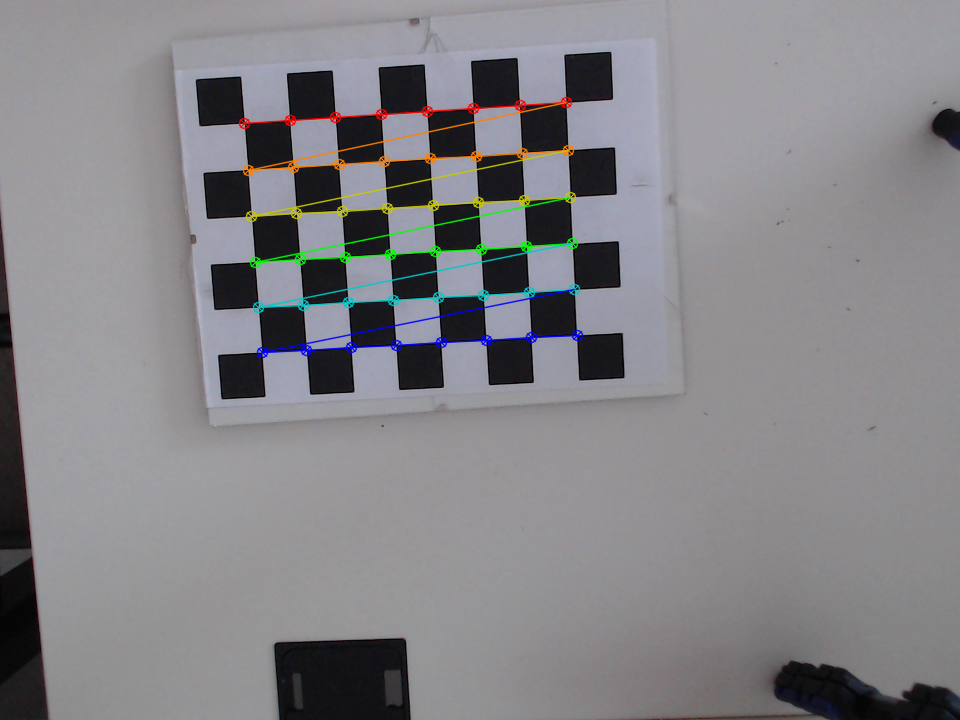
\includegraphics[width=0.32\linewidth]{img/hauptteil/calibration/chessboard_corner_0.png}
			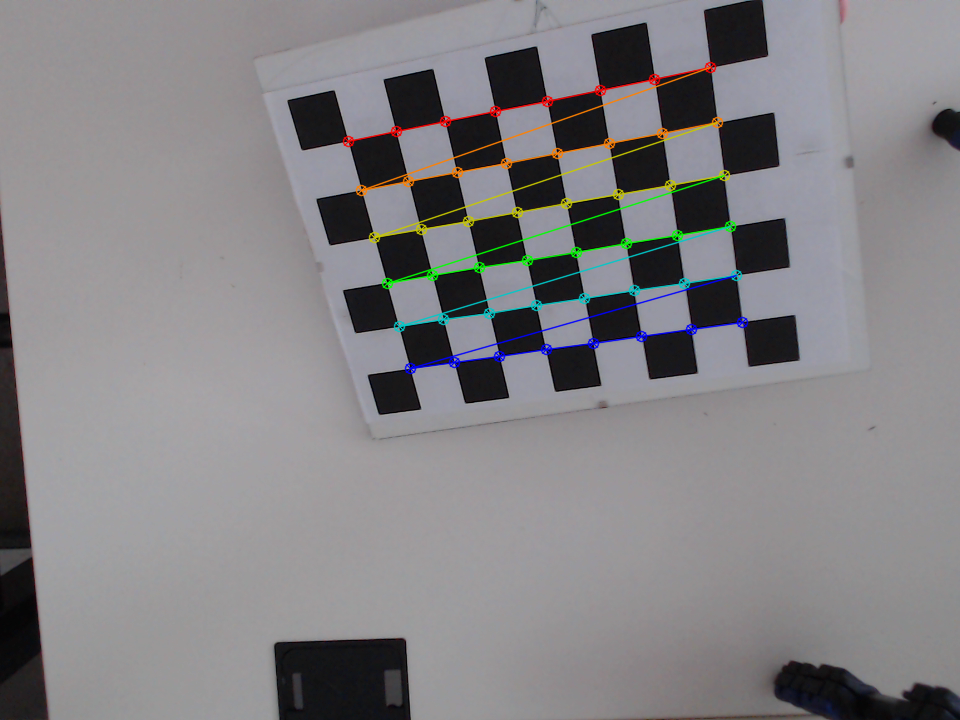
\includegraphics[width=0.32\linewidth]{img/hauptteil/calibration/chessboard_corner_1.png}
			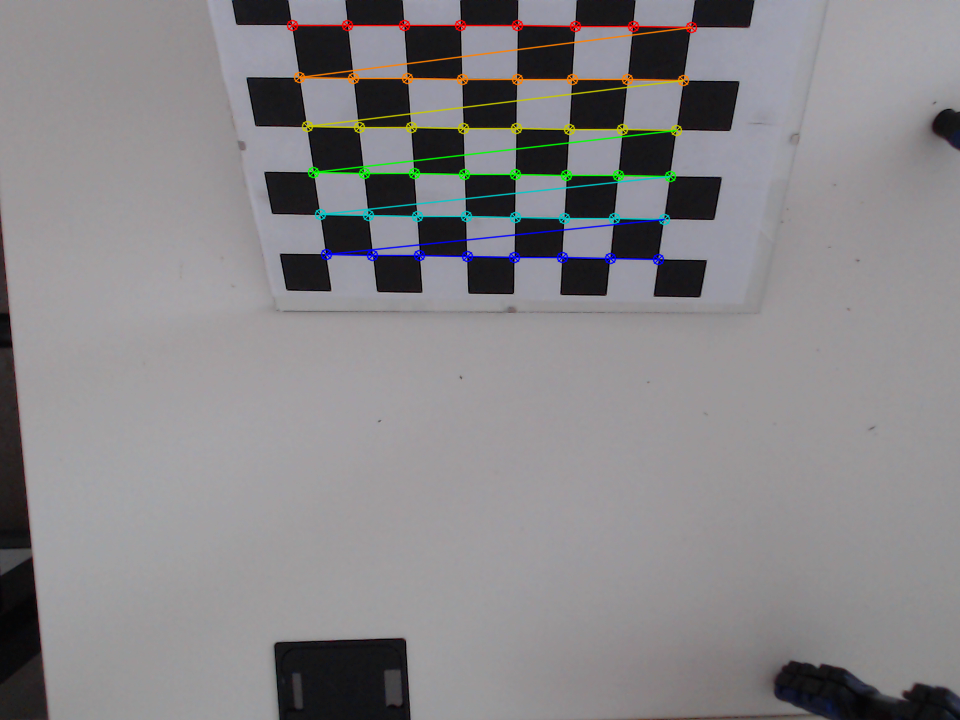
\includegraphics[width=0.32\linewidth]{img/hauptteil/calibration/chessboard_corner_2.png}
			%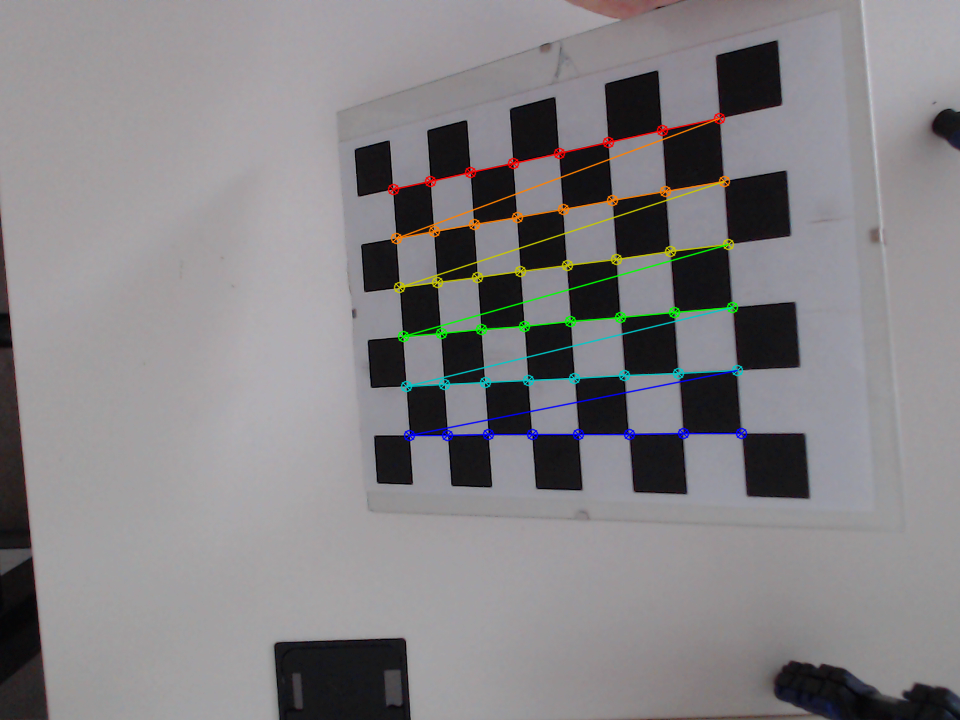
\includegraphics[width=0.39\linewidth]{img/hauptteil/calibration/chessboard_corner_3.png}
			\caption[Schachbrett-Kalibrierung]{Schachbrett-Kalibrierung mit dem Schachbrett aus verschieden Positionen}
			\label{fig:chessboards}
		\end{figure}
	
		Die benutzte Methode heißt \textbf{calibrateCamera()}. Sie nimmt beliebig viele Bilder entgegen. In der eigenen Implementierung wurde gemäß [OpenCv-Cam] vorgegangen. Dabei handelt es sich um die offizielle Einführung zur Kamerakalibrierung von OpenCv.In dem Beispiel in Abb.: (\ref{fig:chessboards}) wurden der Einführung folgend auch die Ecken des definierten Schachbrettes eingezeichnet. Damit kann man im Grunde sichbar machen, dass der Algorithmus das Schachbrett richtig erkannt hat. Gemäß [OpenCv-Cam] werden mindestens 10 Bilder benötigt, um gute Ergebnisse zu liefern. Daran wurde sich ebenfalls gehalten. Die Methode gibt die folgenden Werte zurück:
		
		$\underline{Kameramatrix}$
		
		Die \textbf{Kameramatrix} wird errechnet und ausgegeben. Dabei handelt es sich um die vollwertige Matrix \( A \) aus den Formeln (\ref{eq:basic_trans}) und (\ref{eq:basic_trans_complete}).
		
		$\underline{Distortion-Koeffizienten}$
		
		Die Distortion-Koeffizienten werden gemäß [OpenCv-Cam] geliefert. Distortion bedeutet Verzerrung und bezieht sich auf das aufgenommene Bild. Dies Auswirkungen sind, dass aufgenommene gerade Linien in der Szene im Bild nicht mehr gerade dargestellt werden. Sie biegen sich bzw. sind verzerrt. Es gibt zwei verschiedene Verzerrungen, beschrieben in [Dist] und von OpenCv selbst in [OpenCv-CamCalib].
		
		\begin{figure}[h]
			\centering
			\subfloat[]{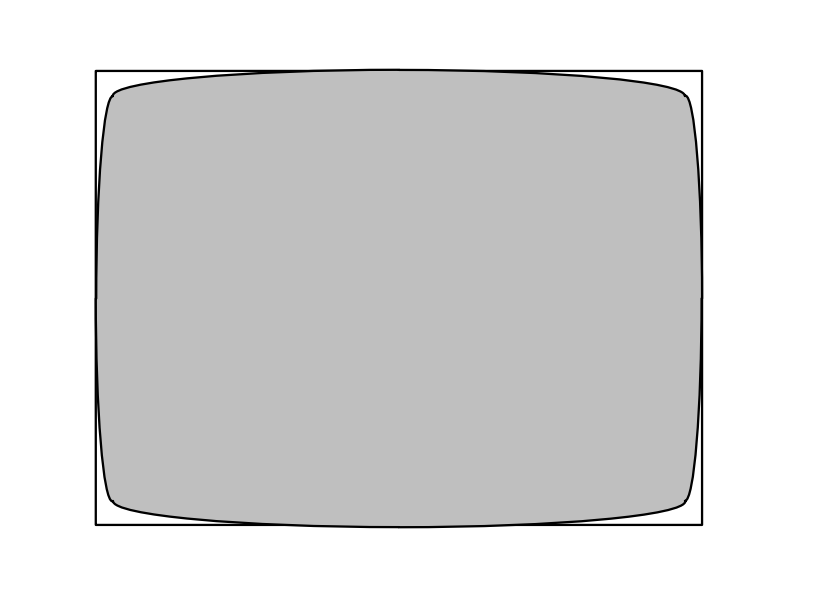
\includegraphics[width=0.4\linewidth]{img/hauptteil/calibration/barrel_dist.png} 	\label{subfig:barrel_dist}} 
			\subfloat[]{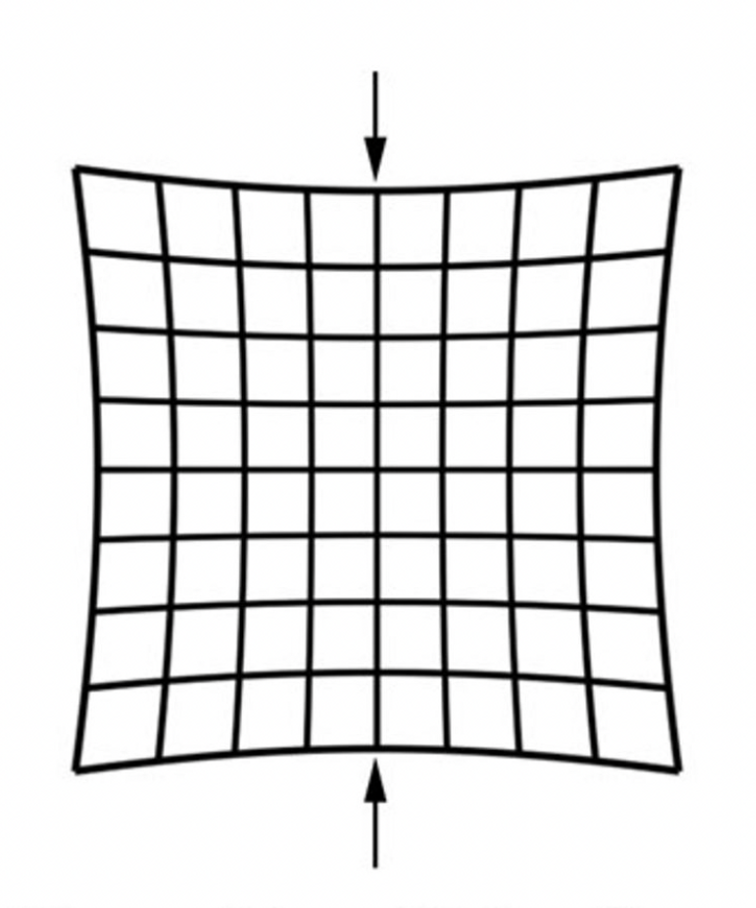
\includegraphics[width=0.4\linewidth]{img/hauptteil/calibration/pinc_dist.png}
				\label{subfig:pinc_dist}}
			\caption[Verzerrung bei Bildern]{Verzerrung bei Bildern; \ref{subfig:barrel_dist} zeigt die Tonnen-Verzerrung (engl.: Barrel-Distortion) und \ref{subfig:pinc_dist} die Kissen-Verzerrung (engl.: Pincushion-Distortion)}
			\captionsource{https://www.learningwithexperts.com/photography/blog/look-out-for-lens-distortion}
			\label{fig:distortion}
		\end{figure}
	
		Um dieser Verzerrung entgegenzuwirken gibt es in OpenCv die Methode \textbf{undistort()}. Diese bringt ein Bild wieder in den normalen Zustand und benutzt dabei die gefunden Koeffizienten [OpenCv-Cam]. Das benutzen dieser Methode ist unumgänglich. Die Laserlinie ist bei einem ebenen Untergrund gerade. Wenn diese allerdings gebogen ist, führt das beim Aufspannen auf die Ebene zu Höhenunterschieden zwischen den Punkten. Die Verzerrung ist nicht Teil des Pinhole Camera Models und somit auch kein Teil der Formel (\ref{eq:basic_trans}). Bevor mit aufgenommenen Bildern gearbeitet wird, werden die jedoch mit der Methode \textbf{undistort()} entzerrt.
		
		\begin{figure}[h]
			\centering
			\subfloat[]{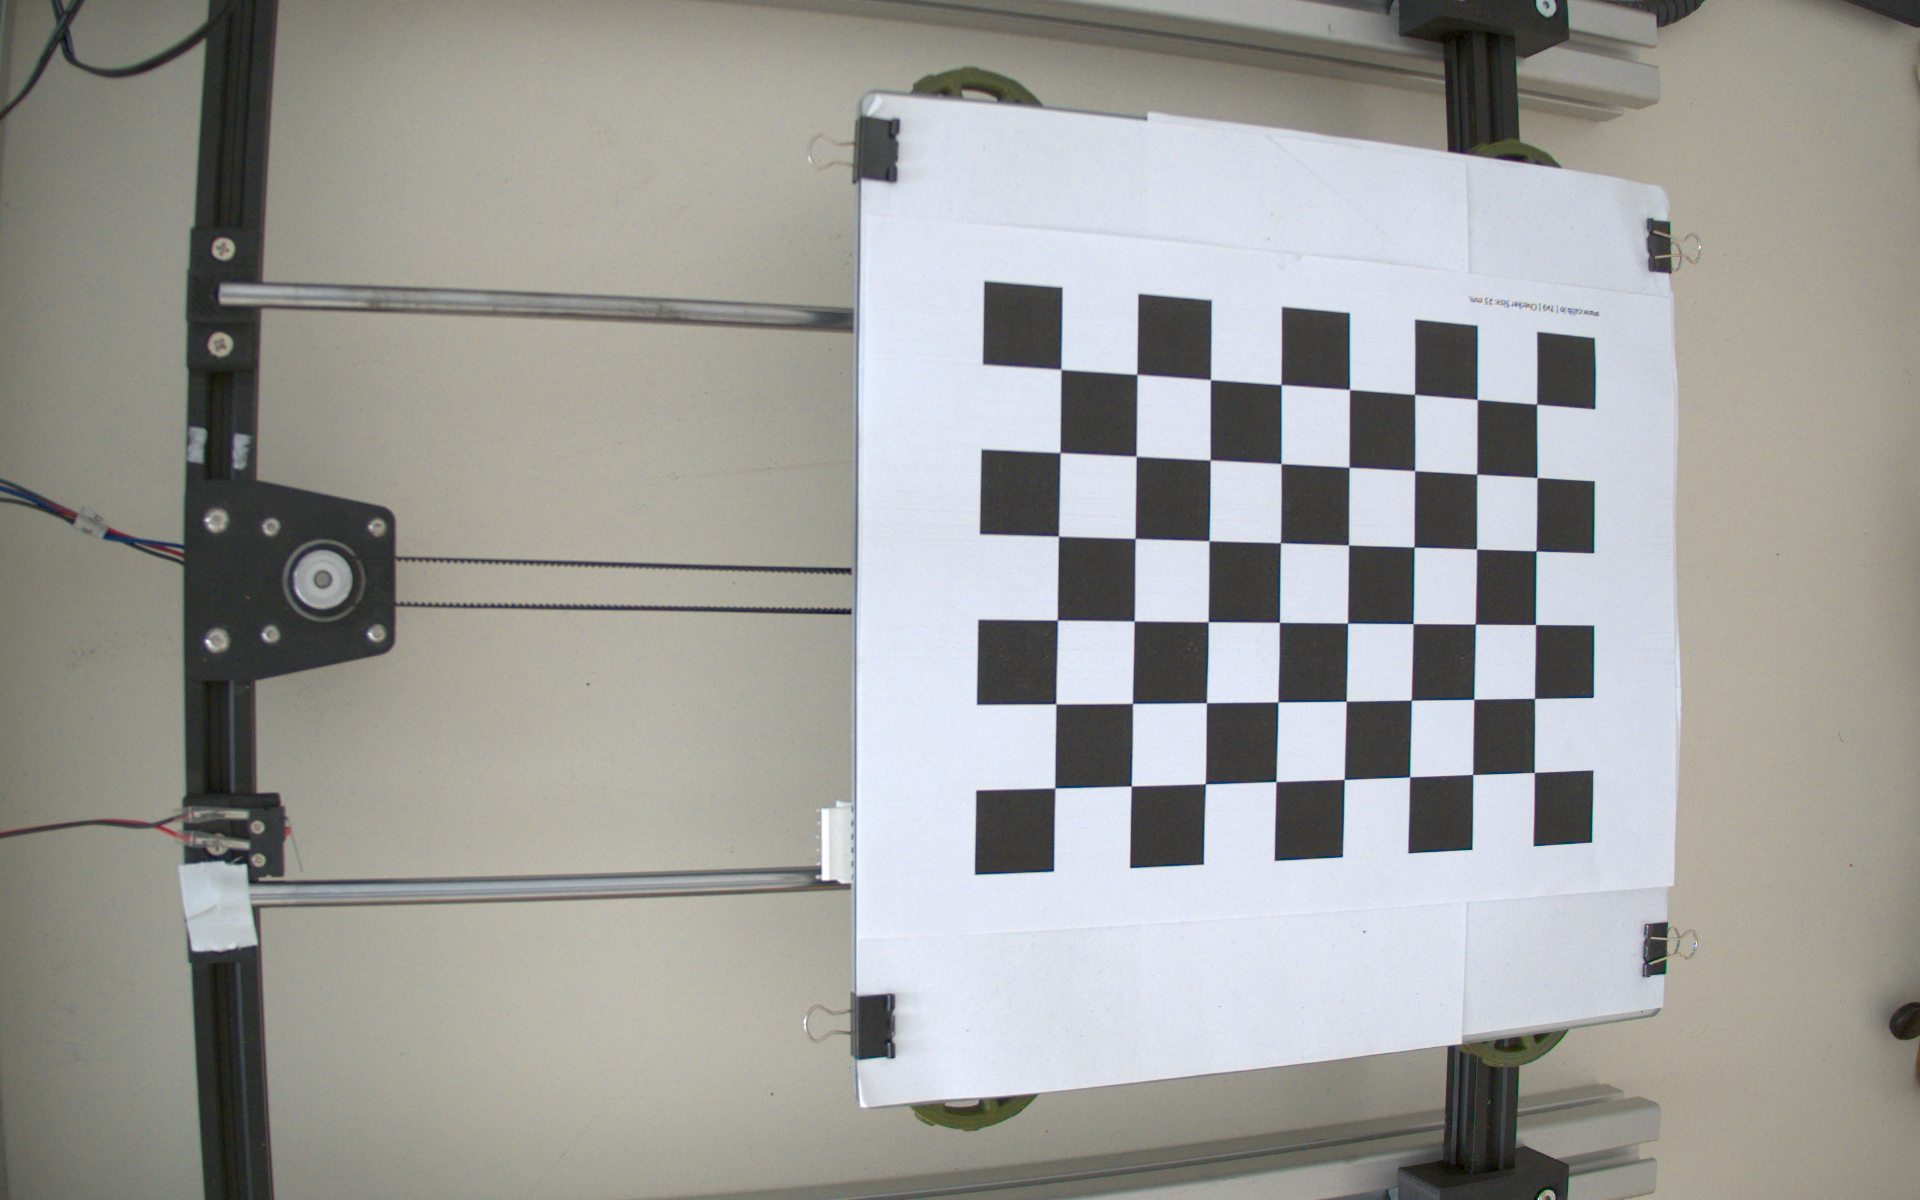
\includegraphics[width=0.49\linewidth]{img/hauptteil/calibration/distorted.png} 	\label{subfig:distorted}} 
			\subfloat[]{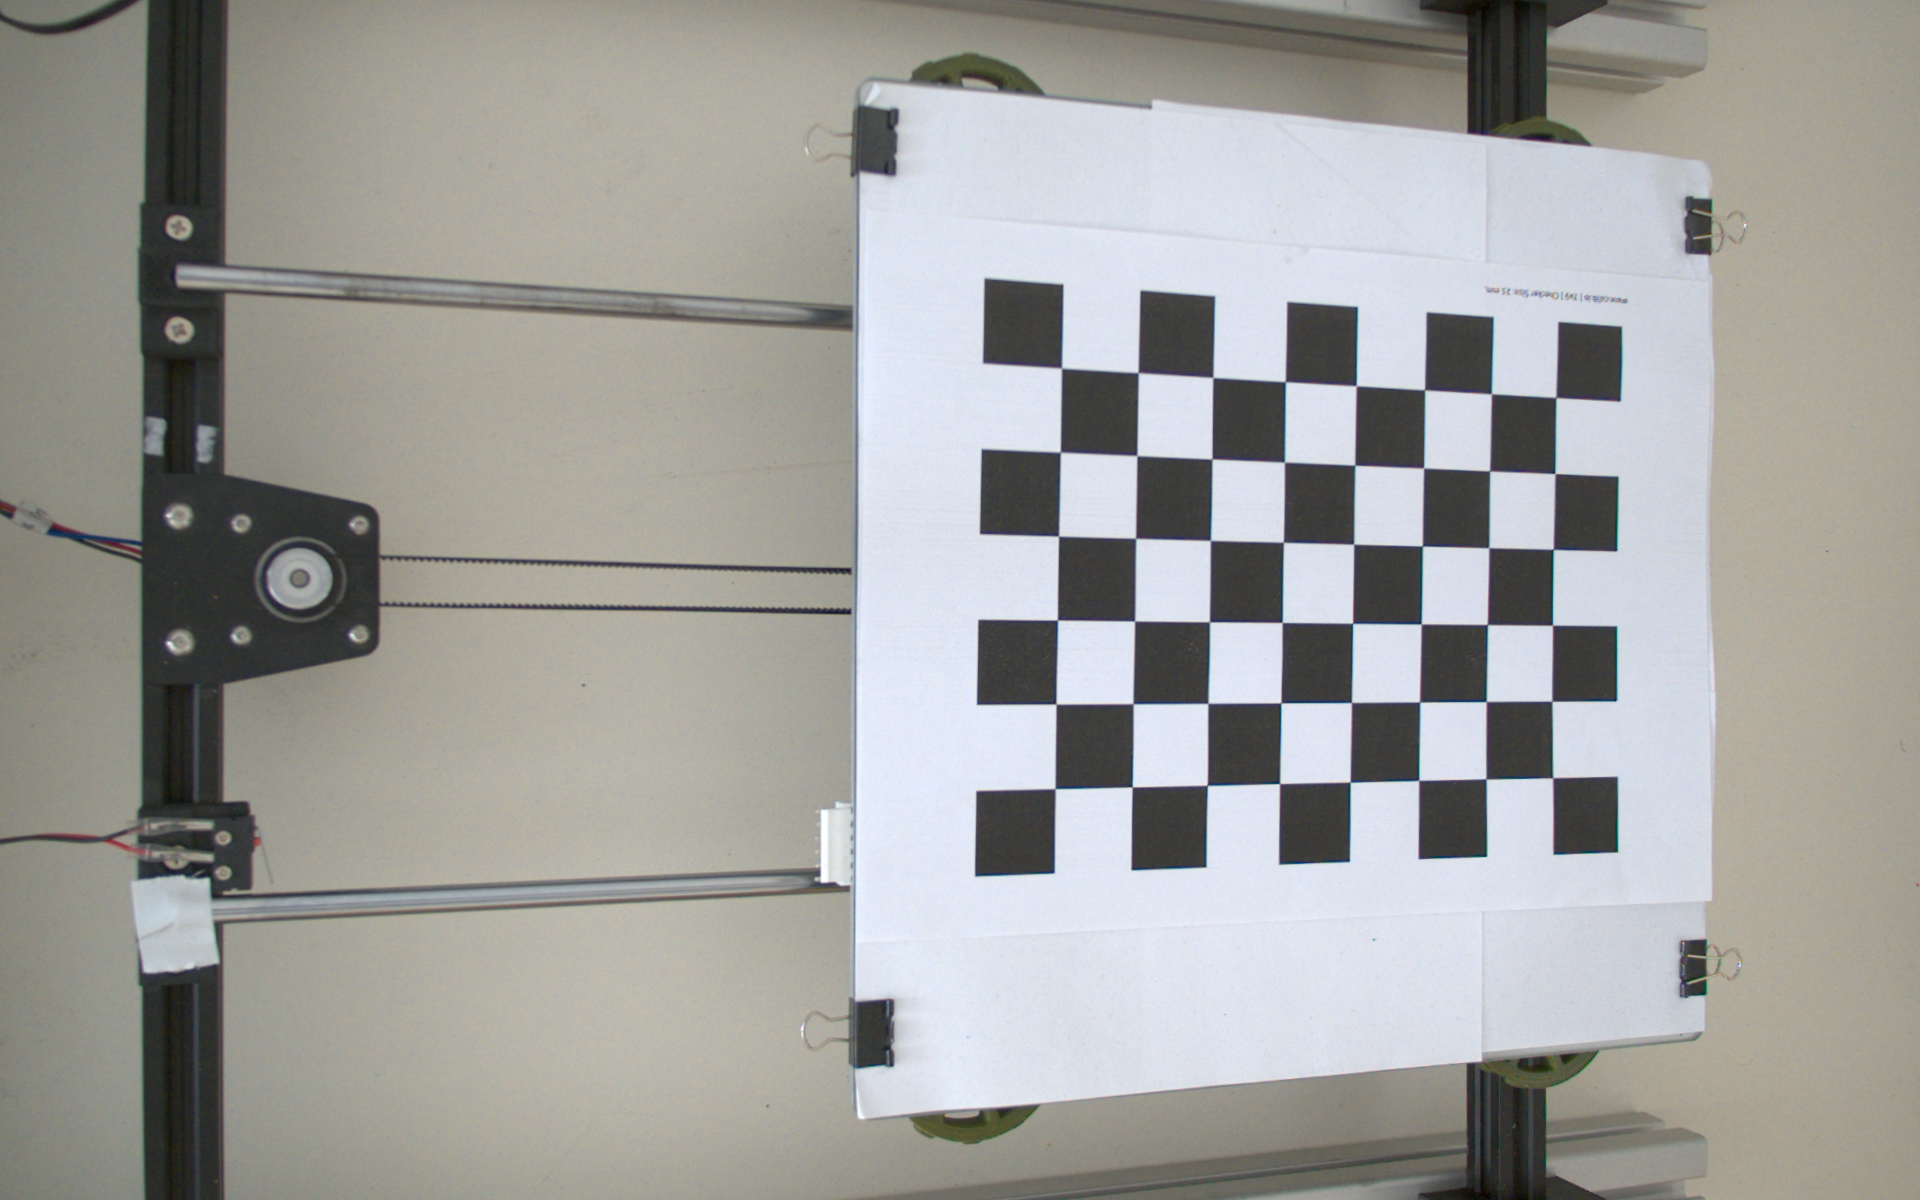
\includegraphics[width=0.49\linewidth]{img/hauptteil/calibration/undistorted.png}
				\label{subfig:undistorted}}
			\caption[Beispiel für die Verzerrung in Bildern]{Hier ein direktes Beispiel aus dem Aufbau. \ref{subfig:distorted} zeigt das Bild vor dem Anwenden von \textbf{undistort()} und \ref{subfig:undistorted} danach.}
			\label{fig:distortion_bsp}
		\end{figure}
	
		Ebenso ist erkennbar, dass es sich bei den verwendeten Kameramodell um eine \textit{Barrel-Distortion} (siehe Abbildung \ref{subfig:barrel_dist}) handelt.
		
		$\underline{Rotationen \; und \; Translationen}$
		
		Die Methode gibt ebenfalls eine Rotationsmatrix und einen Translationsvektor für jedes übergebene Schachbrett zurück. Das sind extrinsische Parameter. In jedes Schachbrett wird ein Koordinatensystem gelegt. Die Rotation und Translation beschreiben dann die Transformation von der Kamera zu diesem Koordinatensystem. Es werden also auch schon extrinsische Parameter geliefert. Diese sind allerdings für den Lasertriangulationssensor selbst nicht ausschlaggebend. Damit dieser mit dem Laser kalibriert werden kann, also eine Ebenen-Gleichung für den Laser gefunden wird, muss der Laser mit auf den Bildern abgebildet sein. Dann kann man die Linie in Bezug auf das gefundene Weltkoordinatensystem weiterverwenden. Für die extrinsische Kalibrierung wurde eine extra Methode entwickelt, welche im nächsten Kapitel beschrieben wird. Die Rotation und Translation zu den verschiedenen Positionen des Schachbrettes sind nicht von Interesse. 
		
		Die intrinsische Kalibrierung ist nur dazu da, die Kameramatrix zu finden und die Distortion-Koeffizienten zu bestimmen, damit die verwendeten Bilder nicht verzerrt sind. Die Kameramatrix ist explizit für die Kamera gültig, mit welcher das Schachbrettmuster aufgenommen wurde. Sie kann also bestimmt werden und ist dann für alle folgenden Rechnungen gültig und unverändert. Genauso verhält es sich mit den Distortion-Koeffizienten. Das bedeutet, dann der Lasertriangulationssensor initial einmal mit dieser Methode kalibriert werden muss, um die intrinsischen Parameter zu bestimmen. Danach werden die Kameramatrix und die Distortion-Koeffizienten abgespeichert und die extrinsische Kalibrierung kann beginnen. 
			\label{chap:kalibrierung_intrinsisch}
			
		\newpage
		\subsubsection{Extrinsische Kalibrierung}
		Die extrinsische Kalibrierung beschäftigt sich allgemein damit die Kamera zu den eingebauten Linienlaser zu kalibrieren. Genauer gesagt geht es nicht konkret um den Laser, sondern die Laserlinie. Ziel dabei ist es, eine Ebenengleichung zu erhalten, die sich im Kamerakoordinatensystem befindet den Laser repräsentiert. Um sich das besser vorzustellen, kann nochmal Abb.: (\ref{fig:lasertriangulation}) eingesehen werden. Hier ist die symbolische Ebene des Lasers rot markiert. Die dazugehörige Gleichung beschreibt dann die Position des Laserlinienstrahls. Grundlegend richtet sich die Methode, um die Ebenen-Gleichung zu finden erneut nach Bajpai und Perelman [baj-per]. \newline
		Bekannt ist, dass durch eine Kamerakalibrierung die Rotation und Translation herausgefunden werden können. Durch die intrinsische Kalibrierung ist die Kameramatrix bekannt. Dabei wurde ein Schachbrett aus verschiedenen Positionen aufgenommen. Ziel ist es nun ein Schachbrett mit einer Laserlinie aufzunehmen. Die allgemeine Transformationsformel (\ref{eq:basic_trans_complete}) kann gelöst werden. Mit dem im Kapitel \ref{chap:bildverarbeitung} vorgestellten Verfahren werden die Pixel, die die Laserlinie abbilden gefunden. Nur diese werden in die Formel (\ref{eq:basic_trans_complete}) eingesetzt. Dabei können jetzt die 3D-Punkte errechnet werden, welche sich in dem Weltkoordinatensystem befinden. Das Weltkoordinatensystem liegt dabei auf dem Schachbrett und ist durch die Rotationsmatrix und den Translationsvektor bestimmt. Aus einer Linie kann jedoch keine Ebene abgeleitet werden. Was ist aber, wenn sich im selben Bild ein zweites Schachbrett befindet, welches nicht eben, sondern in einem gewissen Winkel zu dem ersten befindet. Das zweite Schachbrett hat dabei dann ein eigenes Weltkoordinatensystem. Da jedoch alle Transformationen bekannt sind, ist es möglich die Laserlinien-Punkte des einen Koordinatensystem in das andere zu transformieren. Betrachtet werden nun zwei Laserlinien, die in einem Winkel zueinander in einem einheitlichen Koordinatensystem stehen. Mit dieser Ausgangslage ist es möglich eine Ebene in die Punkte zu legen. Dabei gibt es diverse Möglichkeiten eine Ebene an Punkte zu fitten und alle liefern eine Ebenengleichung. Rein logisch sind sogar nur mindestens drei Punkte notwendig, um in einem dreidimensionalen Raum eine Ebene zu beschreiben. In diesem Fall sind es weitaus mehr Punkte, die zum finden der Ebene berücksichtigt werden können. \newline
		In [baj-per] wird dann bei jedem Durchgang, bei dem eine Laserlinie in eine Punktewolke übersetzt wird, eine aktuelle neue Ebenengleichung erstellt und die Oberflächenpunkte errechnet. Die Ausgangslage ist hier jedoch etwas anders. Die Idee ist es nach der intrinsischen Kalibrierung eine einmalige extrinsische Kalibrierung vorzunehmen. Es wurde schon erwähnt, dass sich Kamera und Laser in ihrer Position zueinander nicht verändern. Damit bleibt auch die Ebenen-Gleichung in Bezug zur Kamera immer gleich. Die einmal  gefundene Ebenengleichung ist also allgemeingültig für den folgenden Scann. Dieser Vorgang der extrinsischen Kalibrierung soll hier nochmal genau beschrieben werden.
		
		$\underline{Zwei \; Schachbretter \; in \; einem \; Bild}$
		
		Um die extrinsische Kalibrierung auszuführen soll also ein Bild von zwei Schachbrettern gemacht werden. Dabei ist es nötig, das sie in einem Winkel zueinander stehen. Das hat den Grund, dass die verschiedenen Laserlinien einen Winkel bilden müssen, um darin eine Ebene zu finden. Der Winkel ist dabei grundsätzlich egal. Jedoch sollte kein zu hoher oder zu niedriger Winkel gewählt werden, damit dieser nicht zu eng bzw. zu flach ausfällt. Zu diesem Zweck wurde eine eigene Unterlage designt.
		
		\begin{figure}[h]
			\centering
			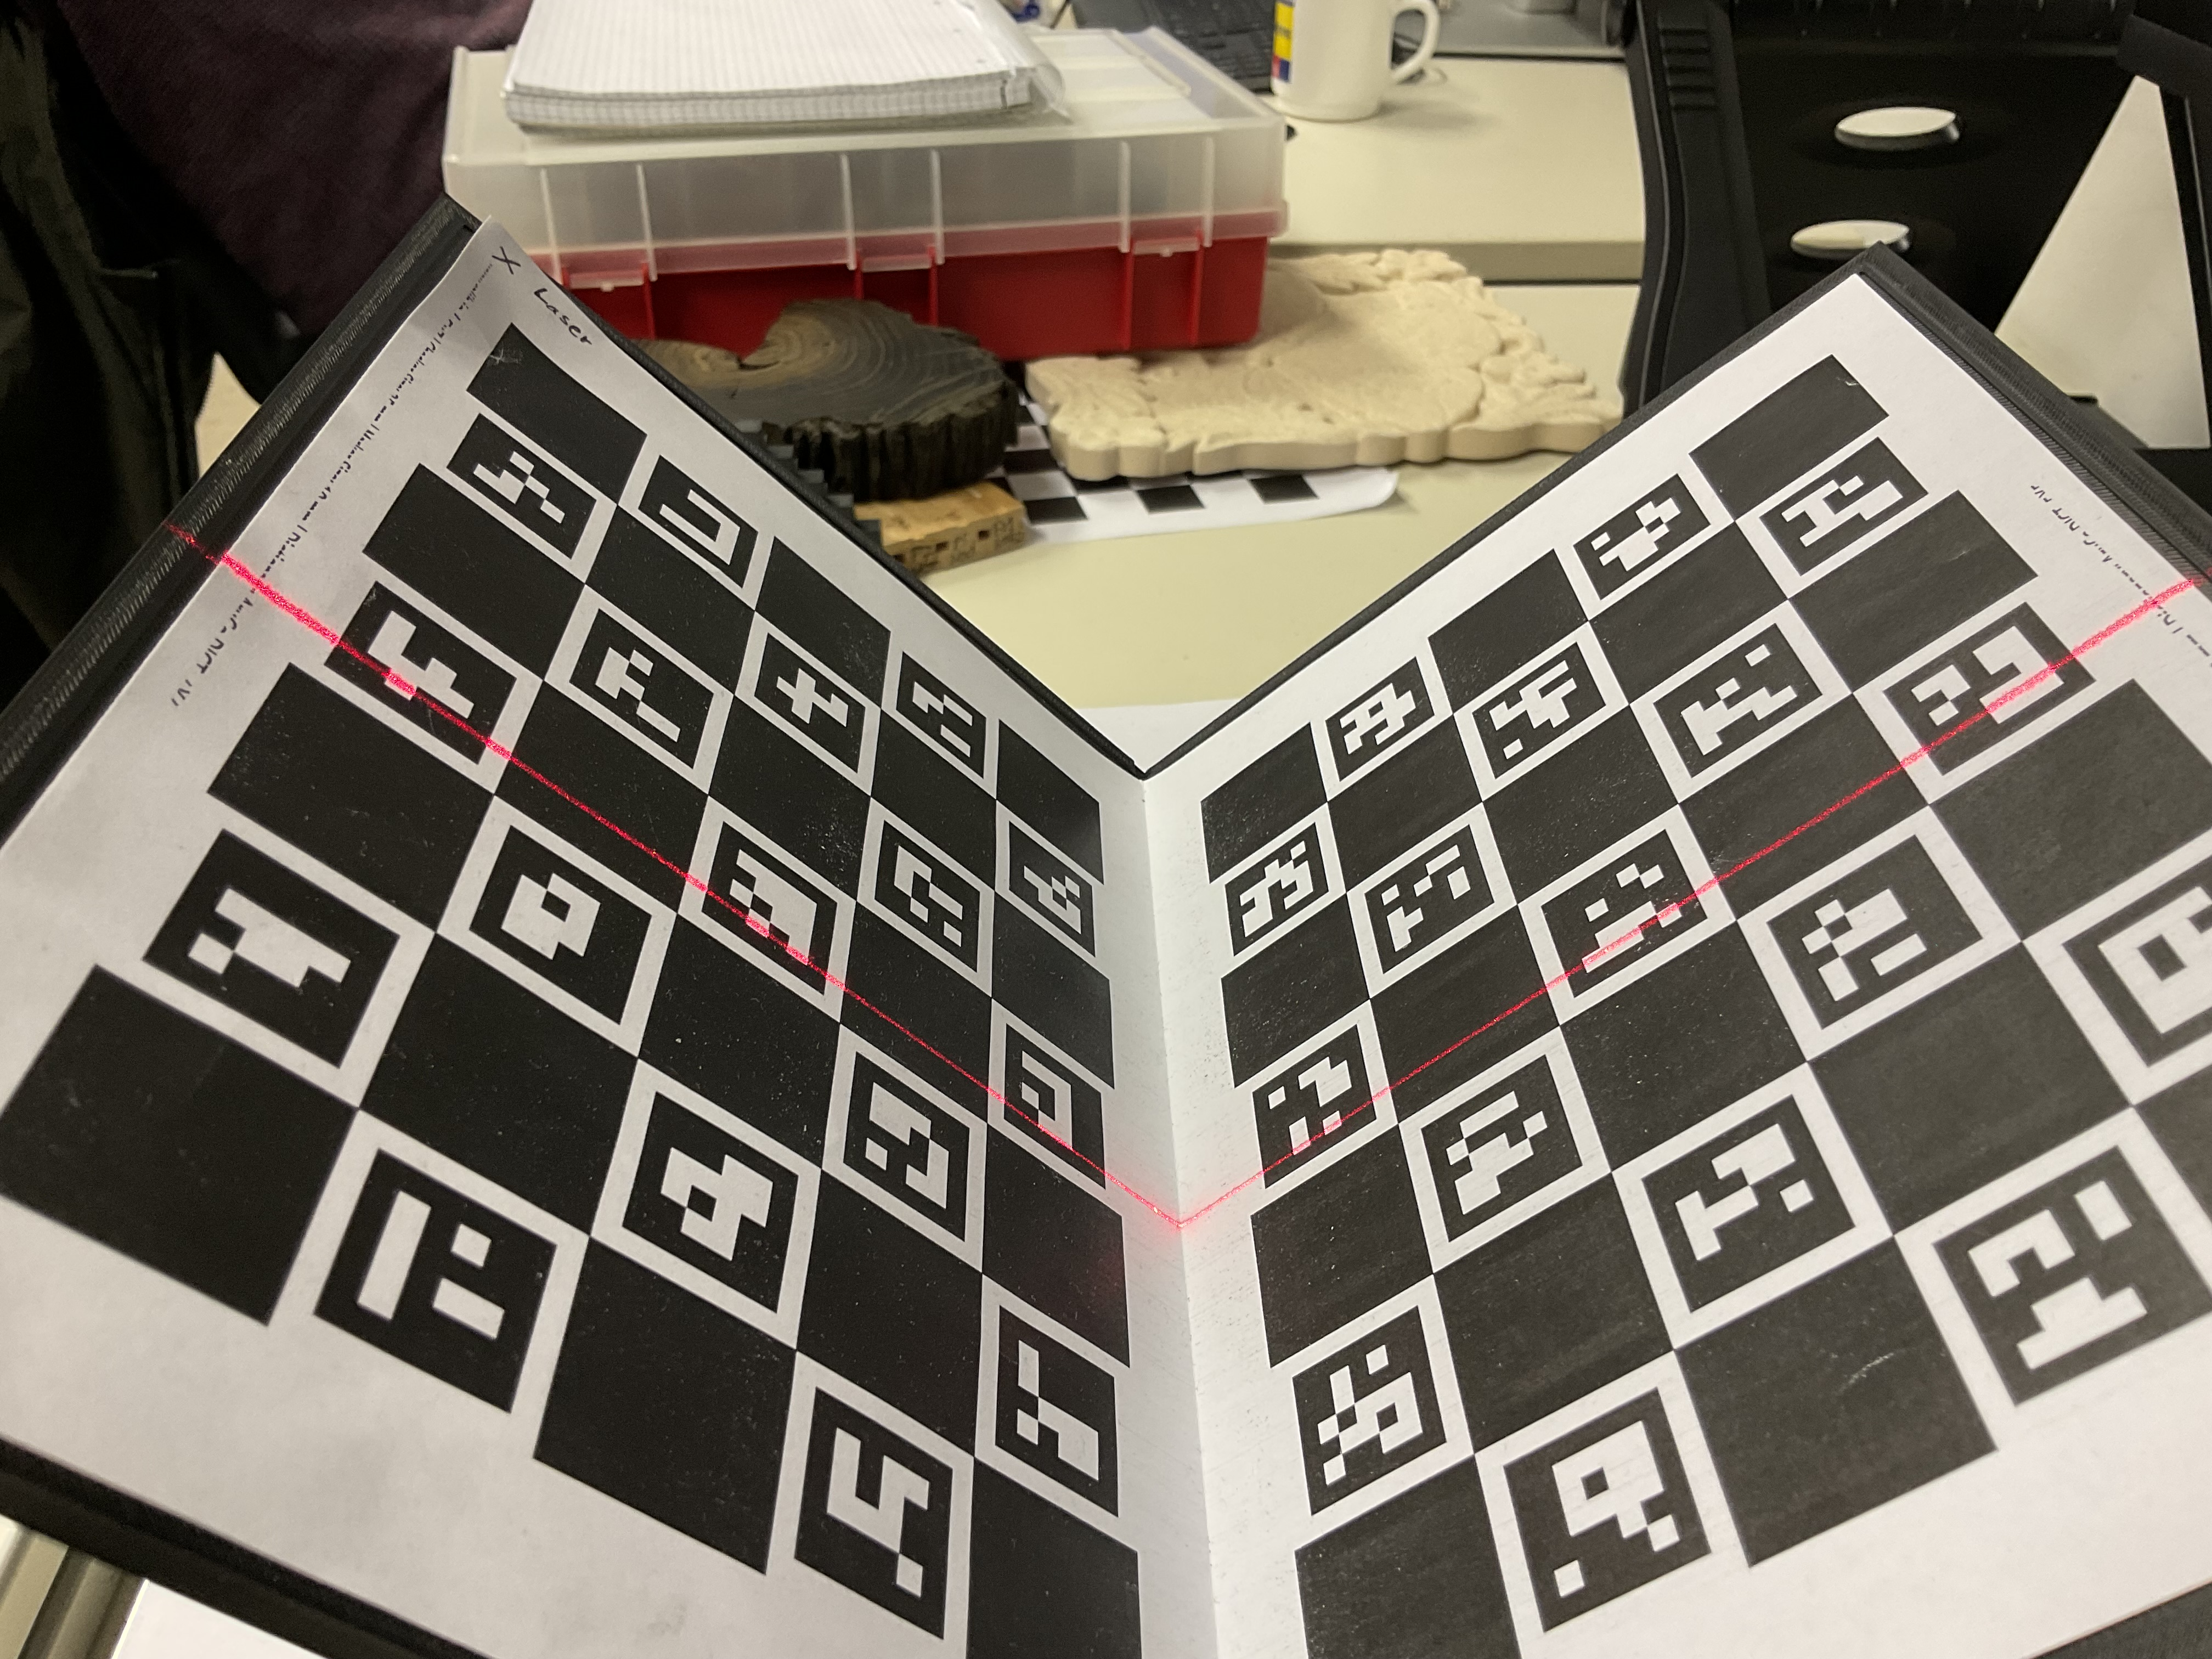
\includegraphics[width=0.49\linewidth]{img/hauptteil/ext-calib/pattern_0.jpg}
			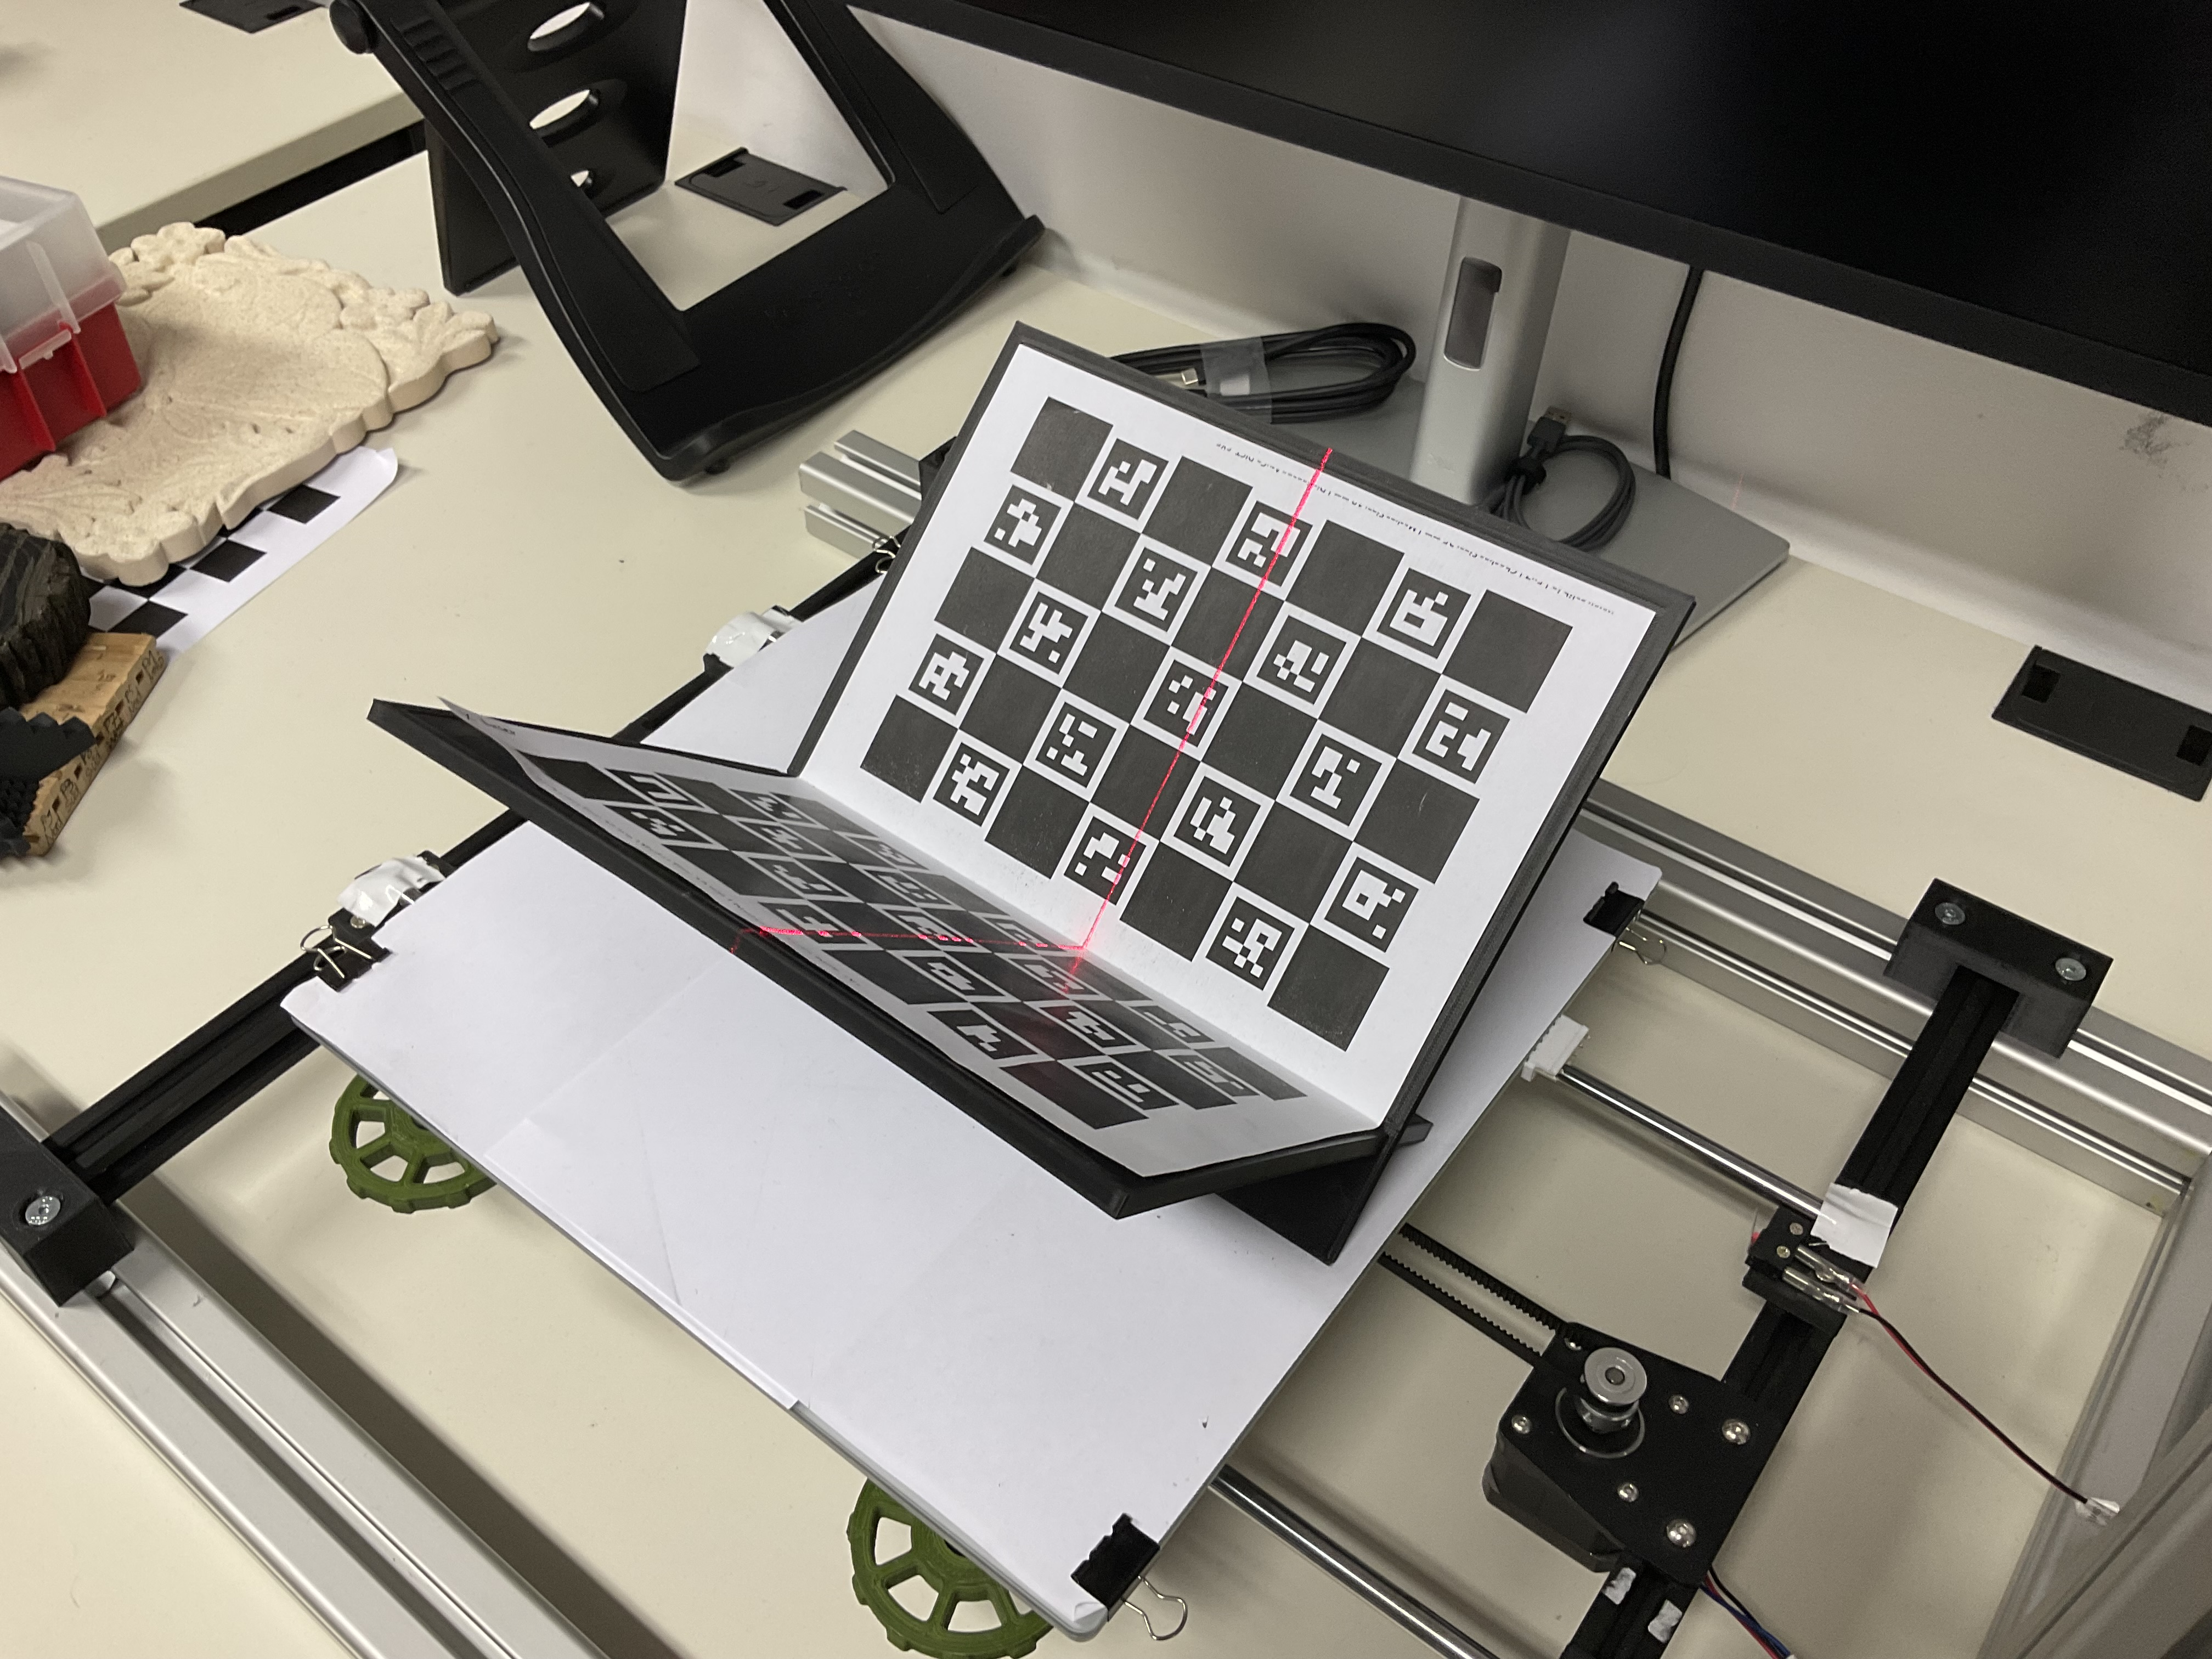
\includegraphics[width=0.49\linewidth]{img/hauptteil/ext-calib/pattern_1.jpg}
			\caption{Unterlage zum Kalibrieren}
			\label{fig:ext-calib-pattern}
		\end{figure} 
	
		In diesem Fall wurde ein 90°-Winkel benutzt. Das Kalibrier-Brett ist über ein 3D-Drucker gedruckt wurden. Diese Bilder sind Beispielbilder. Der entwickelte Lasertriangulationssensor liefert während dem Kalibriervorgang Output-Bilder, die verschiedenen Arbeitsschritte untermalen.
		\begin{figure}[h]
			\centering
			\subfloat[]{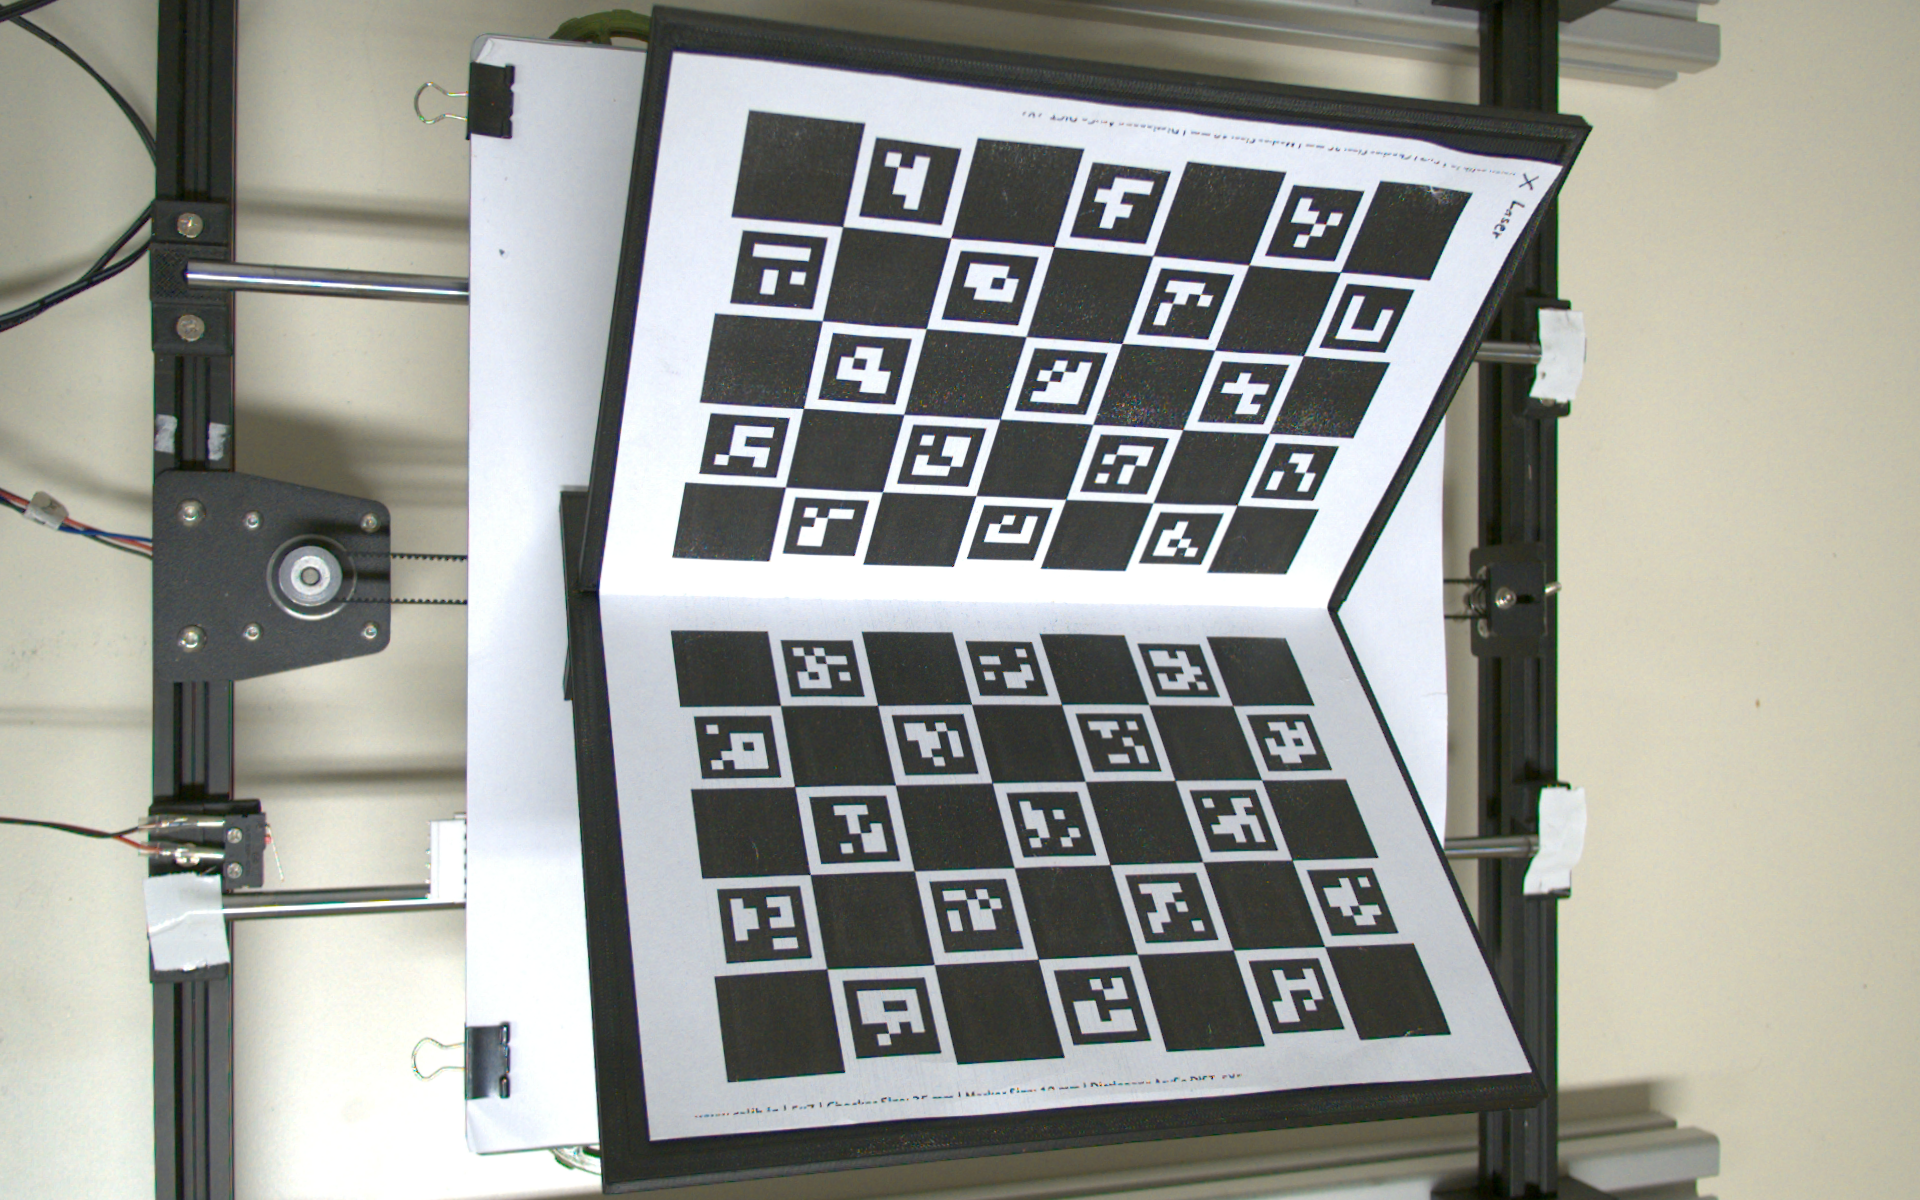
\includegraphics[width=0.49\linewidth]{img/hauptteil/ext-calib/charuco_board.png}
				\label{subfig:raw}}
			\subfloat[]{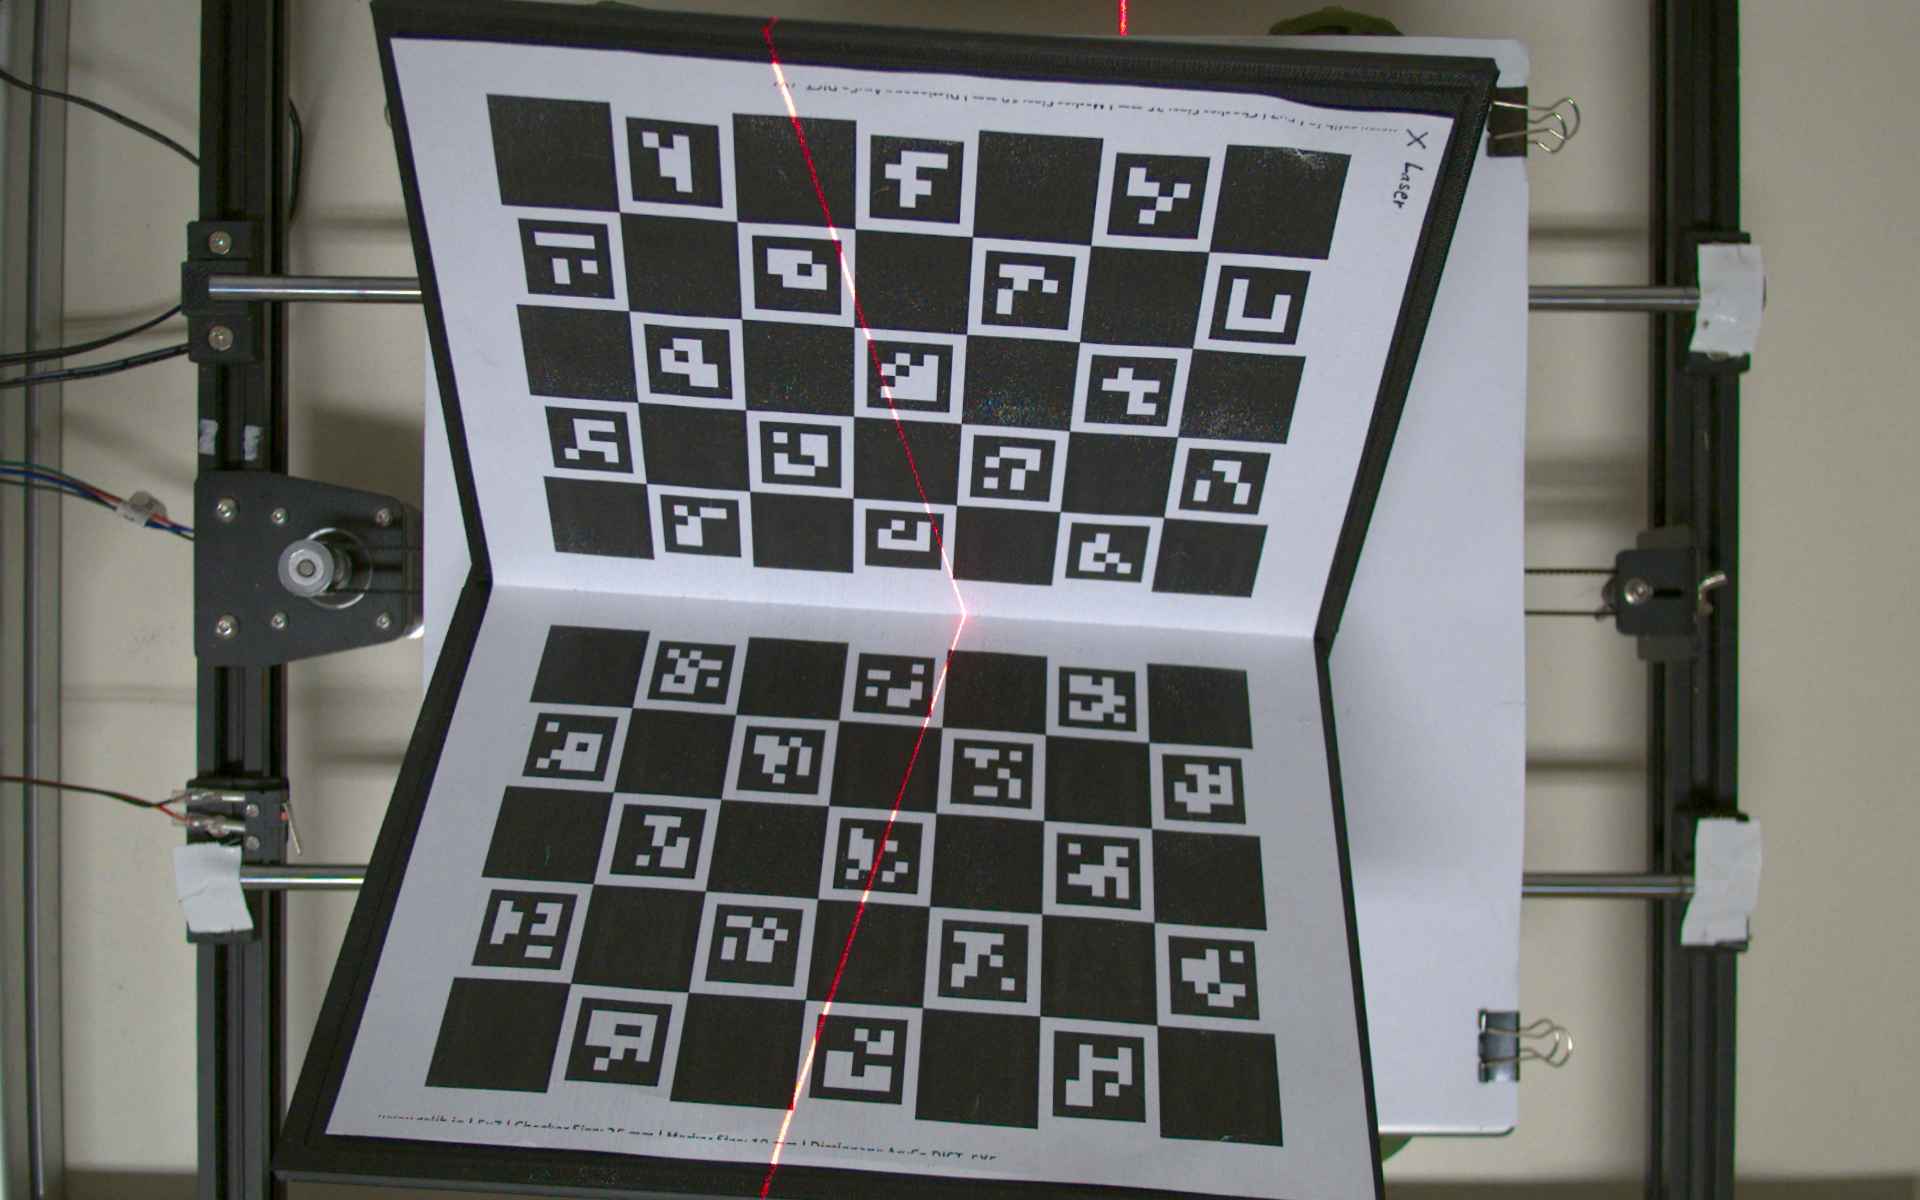
\includegraphics[width=0.49\linewidth]{img/hauptteil/ext-calib/charuco_board_laser.png}
				\label{subfig:raw_laser}}
			\caption{Ausgangsbilder der extrinsischen Kalibrierung}
			\label{fig:ext-calib-raw}
		\end{figure} 
	
		Gemäß Kapitel \ref{chap:bildverarbeitung} wird ein Bild-Paar aufgenommen. In einem ist die Laserlinie sichtbar (Abbildung \ref{subfig:raw_laser})und in dem anderen nicht (Abbildung \ref{subfig:raw}).
		
		$\underline{Unterscheidung \; der \; Schachbretter}$
		
		In den Vorherigen Abbildungen fällt auf, dass es sich bei den verwendeten Kalibriermuster nicht um ein herkömmliches Schachbrett handelt. Das verwendete Muster ist ein ChArUco-Board. Das Problem bei einem herkömmlichen Schachbrett ist, dass der Algorithmus für die Kamera-Kalibrierung in einem einzigen Bild nicht zwischen zwei Schachbrettern unterscheiden kann. Ein ChArUco-Board besitzt in den normal weißen Flächen eines Schachbretts sogenannte ArUco-Marker. Diese Marker können von der Kamera erkannt und eindeutig unterschieden werden. Das finden und unterscheiden der ChArUco-Board ist in OpenCv implementiert. Dabei definiert man, ähnlich zu dem Schachbrett aus der intrinsischen Kalibrierung \ref{chap:kalibrierung_intrinsisch}, im Vorhinein die Parameter des Boards. Dazu gehören nicht nur die Kachel, sondern auch eine gewisse ArUco-Bibliothek, welche die Marker beschreibt. Der Algorithmus kann nun in einem Bild die beiden Boards unterscheiden und platziert ein Koordinatensystem darauf. Vorausgesetzt wird dabei, das die Kameramatrix und die Distortion-Koeffizienten bereits bekannt sind. Da die intrinsische Kalibrierung initial durchgeführt wird, ist diese Voraussetzung erfüllt.  
		
		\begin{figure}[h]
			\centering
			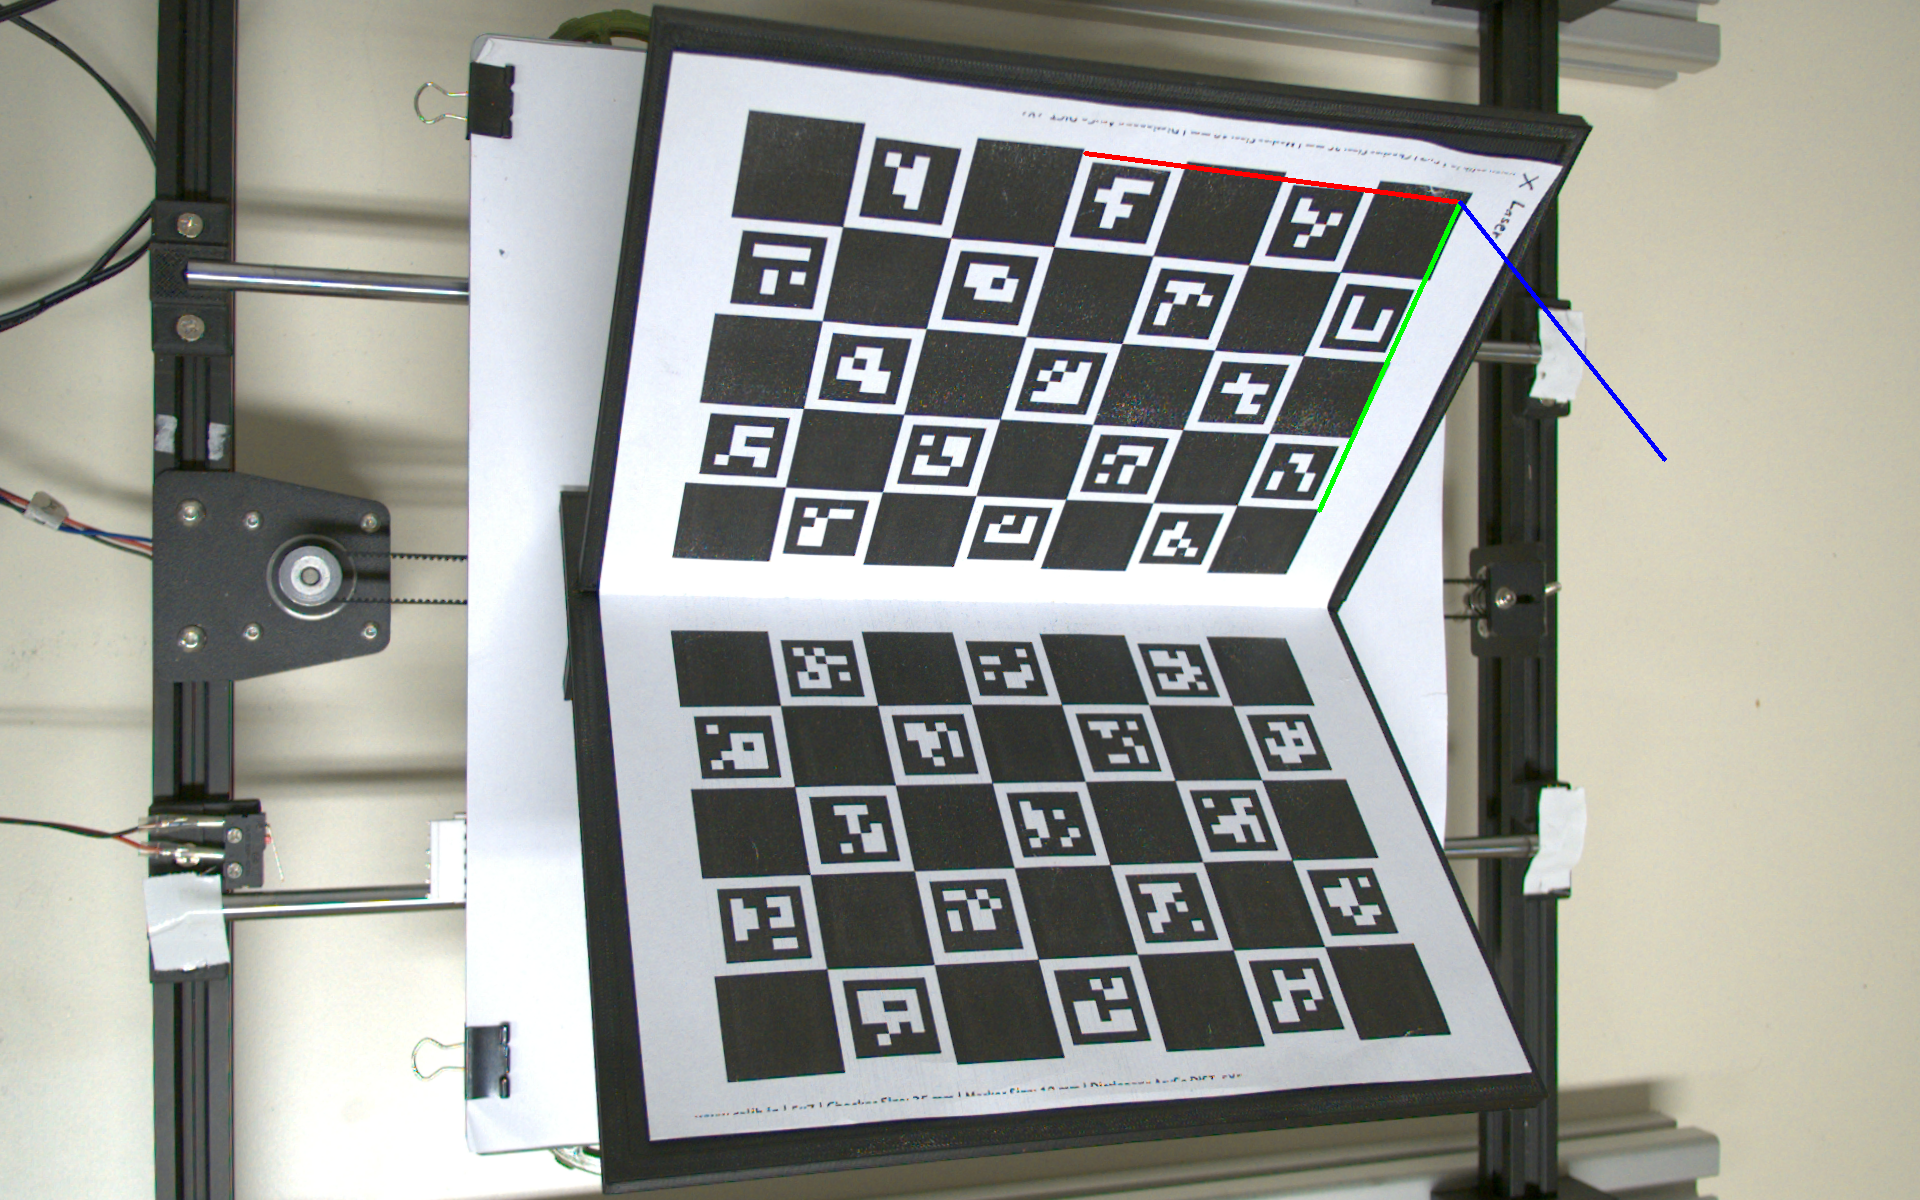
\includegraphics[width=0.49\linewidth]{img/hauptteil/ext-calib/charuco_primary.png}
			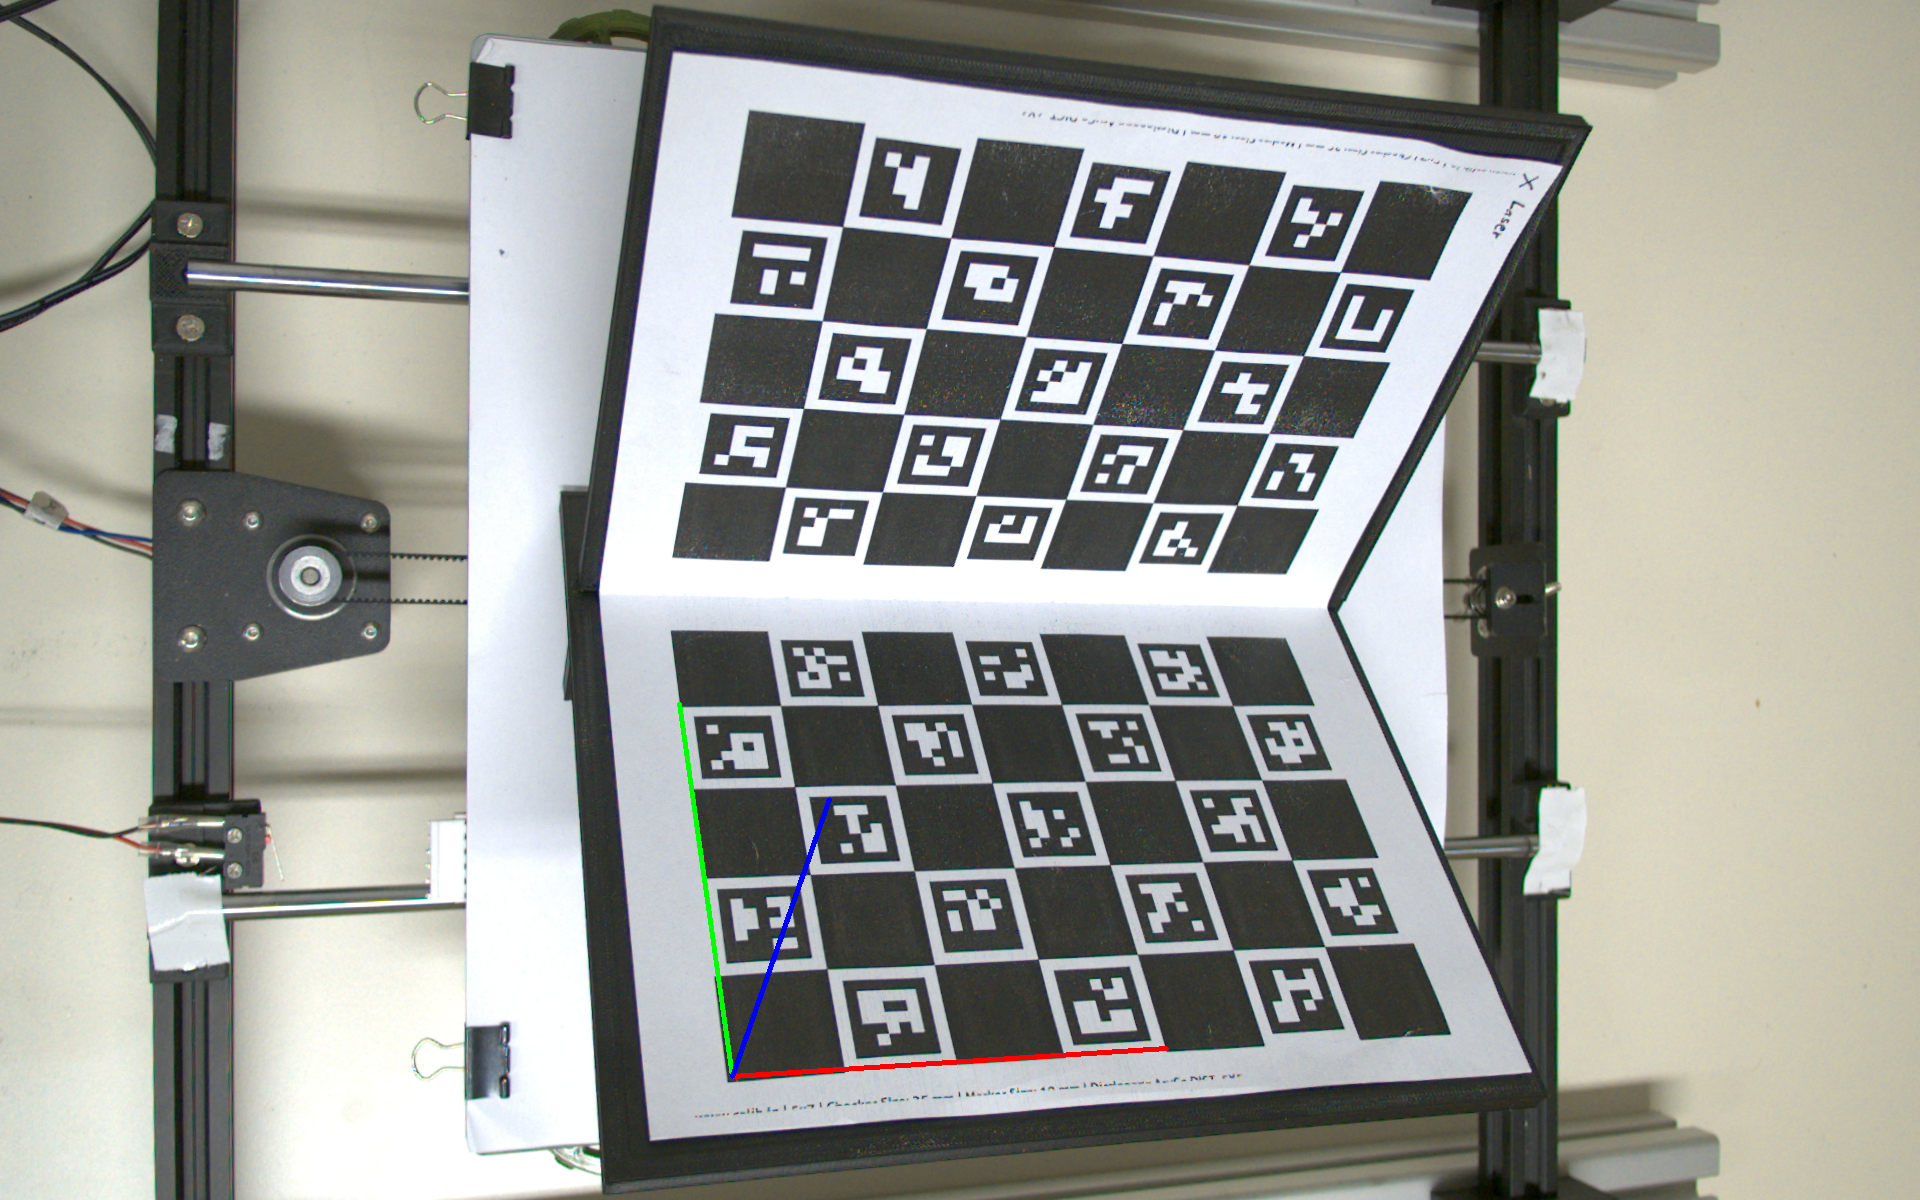
\includegraphics[width=0.49\linewidth]{img/hauptteil/ext-calib/charuco_secondary.png}
			\caption{Weltkoordinatensysteme im ChArUco-Board}
			\label{fig:ext-calib-poses}
		\end{figure}
	
		Bekannt sind jetzt die Rotation und Translation von dem Kamerakoordinatensystem zu den zwei Weltkoordinatensystemen, die aus den ChArUco-Boards folgen.
		
		$\underline{Finden \; der \; richtigen \; Laserlinie}$
		
		Der nächste Schritt muss es sein, die Laserlinie im Bild herauszuarbeiten. Wir wollen die 2D-Punkte der Laserlinie wissen und sie in die 3D-Repräsentation in dem Weltkoordinatensystem umwandeln. Kapitel \ref{chap:bildverarbeitung} beschreibt die Methodik. Das Problem ist, dass nur der Teil der Laserlinie benutzt werden darf, der sich auch tatsächlich auf den jeweiligen Schachbrett befindet. Das bedeutet, dass nur ein gewisser Ausschnitt aus dem Bild wichtig ist. Und zwar genau das zu untersuchende ChArUco-Board. \newline
		Das ChArUco-Board selbst ist dabei die Lösung des Problems. OpenCv erkennt die sowohl die ArUco-Marker als auch die Ecken der Kachel. Dabei besitzen alle eine eindeutige ID. Über die Ecken kann also ein Bereich abgesteckt werden.
		
		\begin{figure}[h]
			\centering
			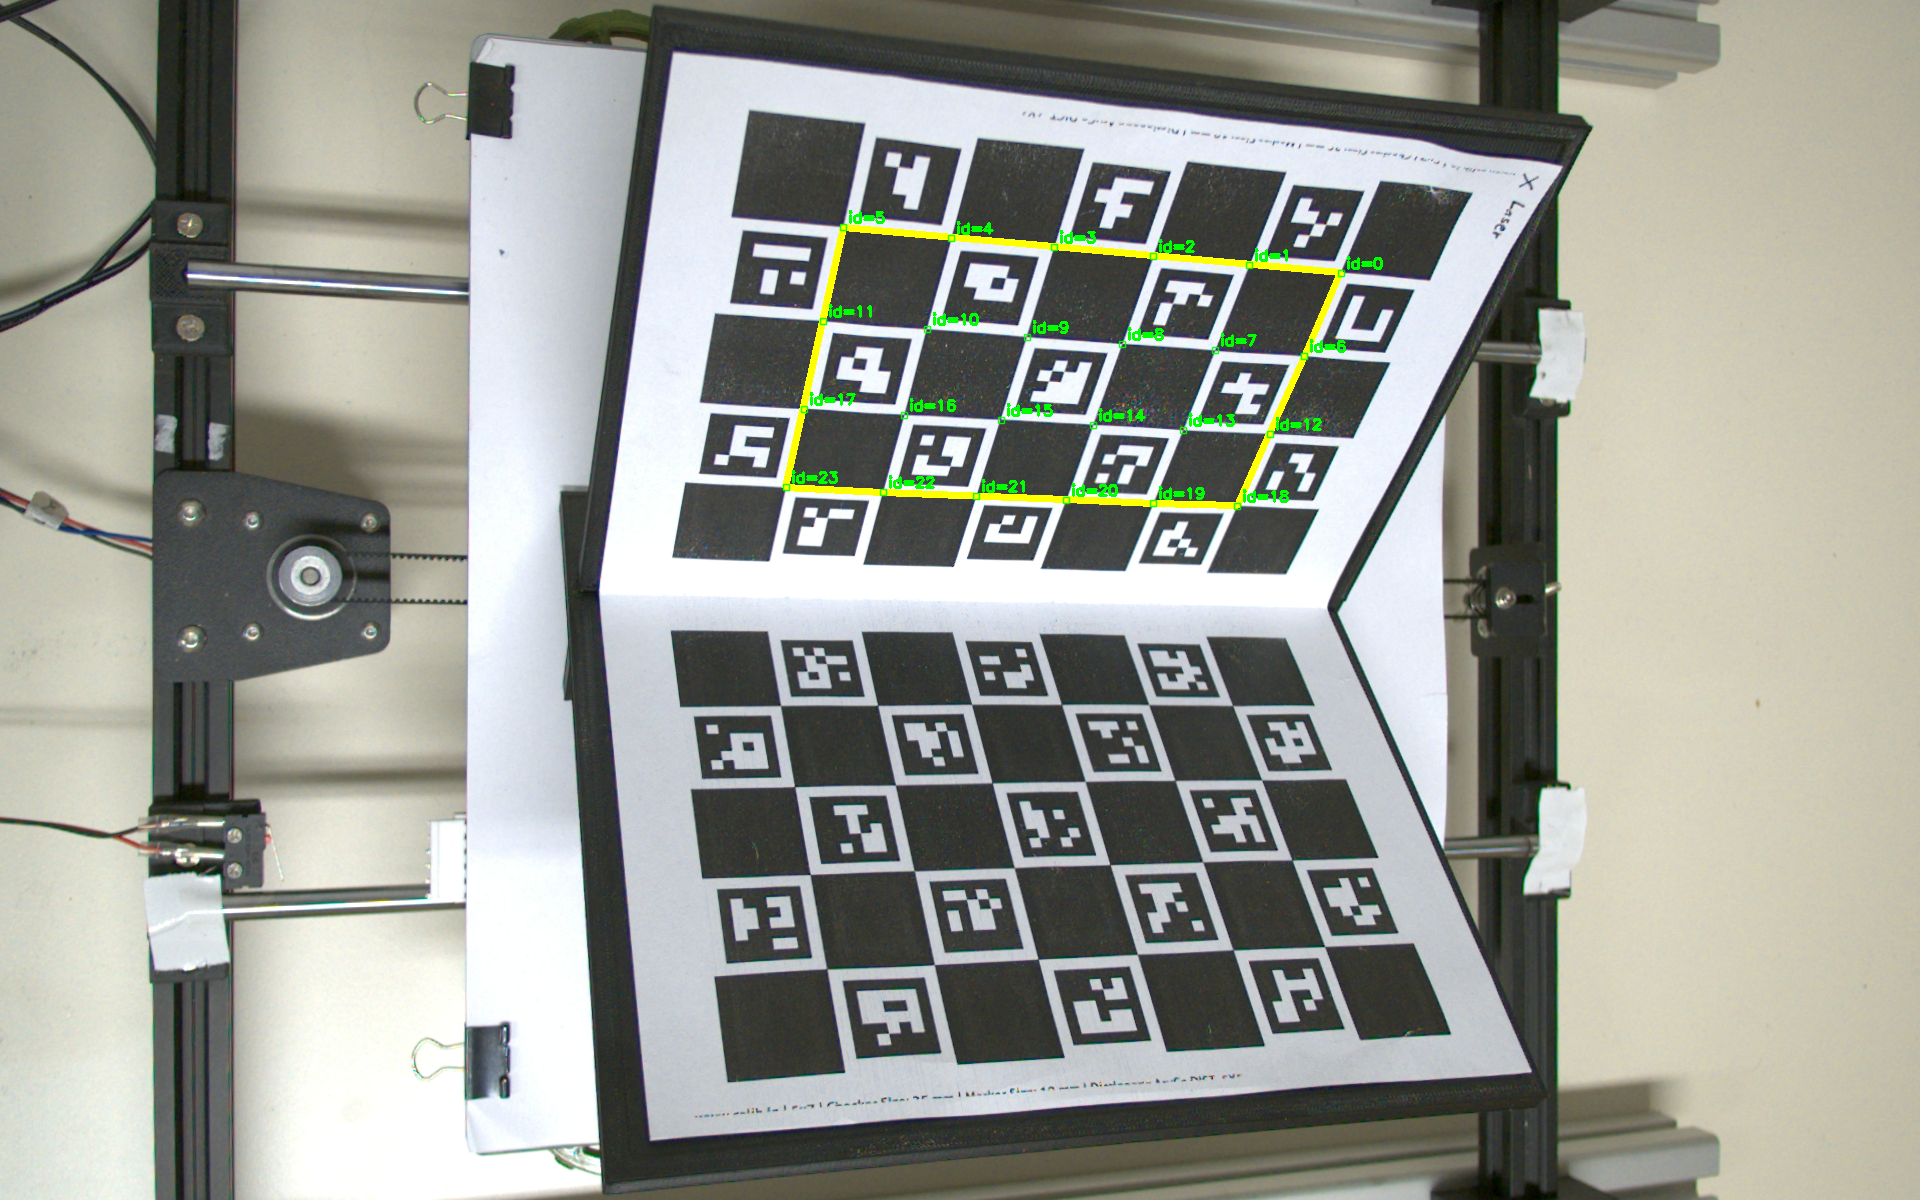
\includegraphics[width=0.8\linewidth]{img/hauptteil/ext-calib/charuco_convex_hull_primary.png}
			\caption{Point of Interest im Bild}
			\label{fig:ext-calib-hull}
		\end{figure}
	
		Um den wichtigen Bereich abzustecken sind die Eckpunkte des Bereiches mit den IDs 0, 5, 18 und 23 ausschlaggebend. Wegen Fehleranfälligkeit wurde jedoch davon abgesehen, genau diese Ecken anzusprechen. Falls in einem Bild eine der äußeren Ecken nicht erkannt wurde, könnten man so den Bereich nicht abstecken. Deswegen wird eine Konvexe Hülle benutzt. Damit werden immer die äußersten Punkte berücksichtigt. Fall gewisse Ecken wegen einer Unschärfe im Bild nicht erkannt werden, führt das nun nicht zu Fehlern. In Abb. (\ref{fig:ext-calib-hull}) ist die abgesteckte Fläche in Gelb eingezeichnet. Falls keine Ecke bzw. keine ID gefunden wurden, ist kein ChArUco-Board erkennbar und die Kalibrierung bricht ab. \newline
		Mit den Bekannten Bereich kann eine Maske entwickelt werden, die auf das Bild angewandt werden kann. Die Maske besteht dabei aus einem schwarzen Bild, in dem der ausschlaggebende Bereich aus weißen Pixeln besteht. Wenn man das Ziel-Bild bitweise mit der Maske verundet, bleibt nur der markierte Bereich im bestehen. Alle andern Pixel sind schwarz. Ausgehend von den Ursprungsbildern (Abb. \ref{fig:ext-calib-raw}) werden für die verschiedenen ChArUco-Boards eine Maske entwickelt und angewandt. Das Ergebnis ist die folgende Abbildung.
		
		\begin{figure}[h]
			\centering
			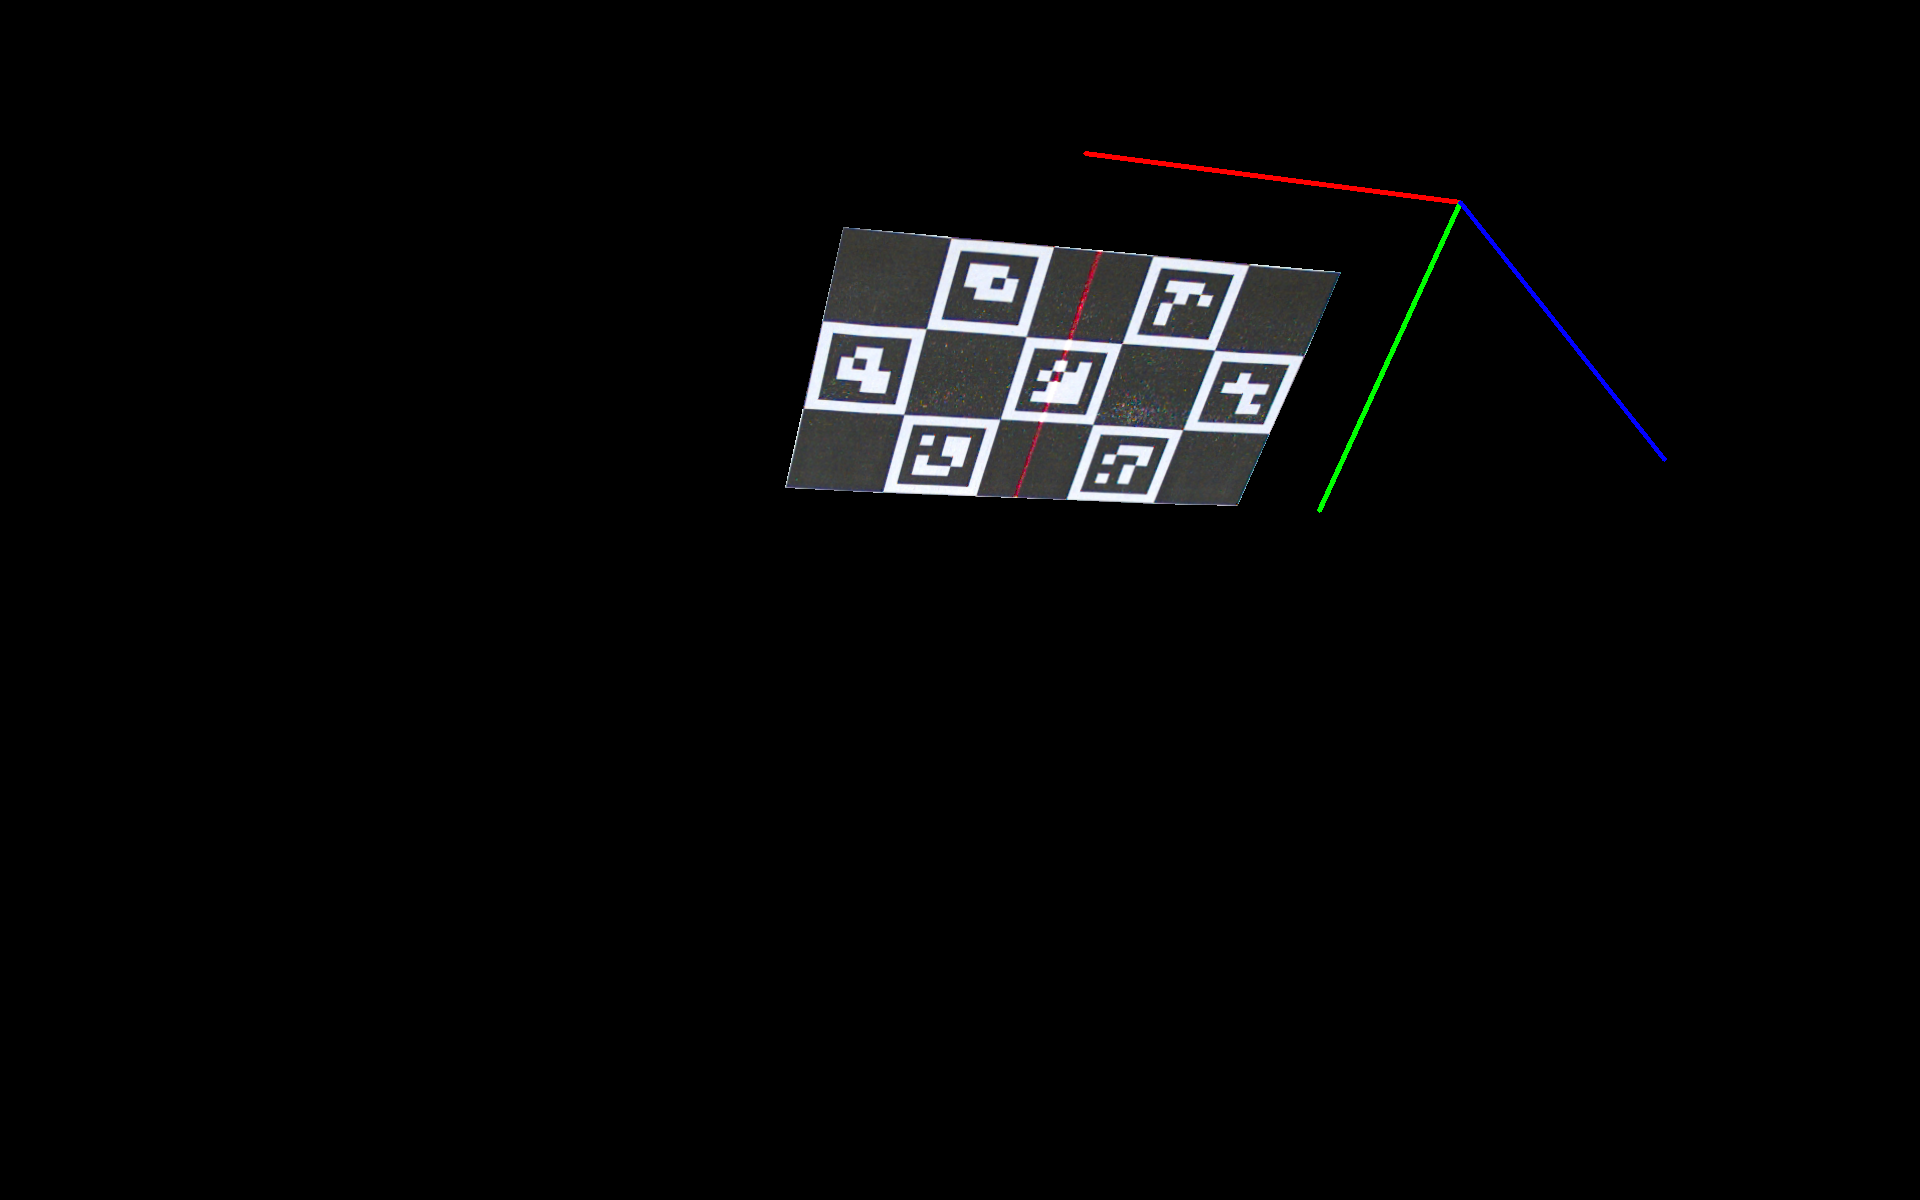
\includegraphics[width=0.49\linewidth]{img/hauptteil/ext-calib/charuco_cut_primary.png}
			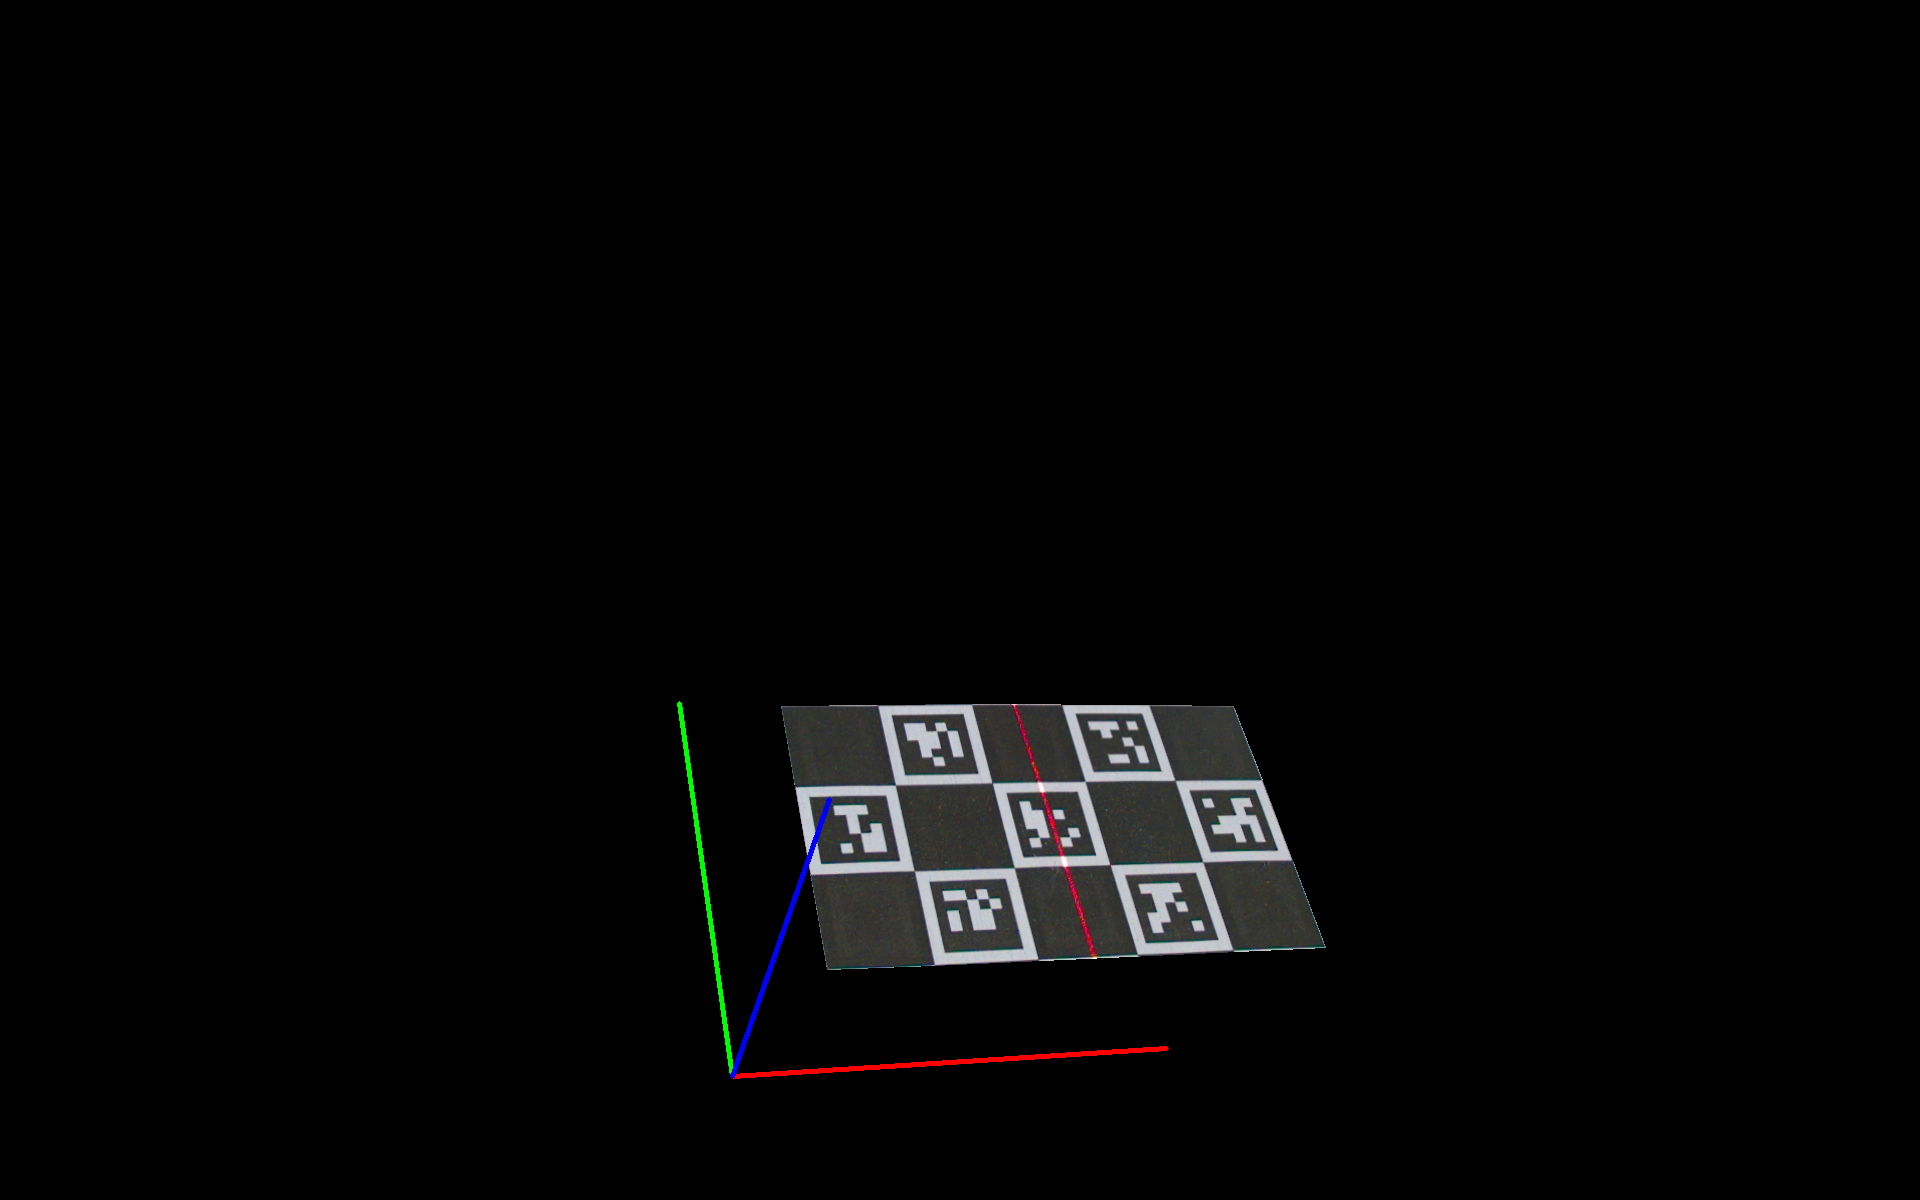
\includegraphics[width=0.49\linewidth]{img/hauptteil/ext-calib/charuco_cut_secondary.png}
			\caption{Ausgeschnitten Laserlinien}
			\label{fig:ext-calib-cut}
		\end{figure}
	
		Die Achsen des jeweiligen Koordinatensystems sind dabei nur zu Übersicht eingezeichnet und nicht Teil der Bildverarbeitung. Verdeutlicht werden soll jedoch, dass das Weltkoordinatensystem bekannt ist. \newline
		Die erstellte Maske kann auch auf das Ursprungsbild ohne Laser angewandt werden. Die beiden ausgeschnittenen Bilder werden an den Algorithmus zum Finden der Laserlinie (Kapitel \ref{chap:bildverarbeitung}) weitergegeben. Die nächste Abbildung zeigt das Ergebnis des Subtrahierens der Bilder. Zur Übersicht sind wieder die Koordinatenachsen eingetragen. Tatsächlich sind an diesem Punkt als Ergebnis der Bildverarbeitung schon die Subpixel der Laserlinie bekannt. Subpixel sind schwierig in einem Bild darzustellen, deshalb wurde sich für das Zeigen des Zwischenschritts entschieden.
	
		\begin{figure}[h]
			\centering
			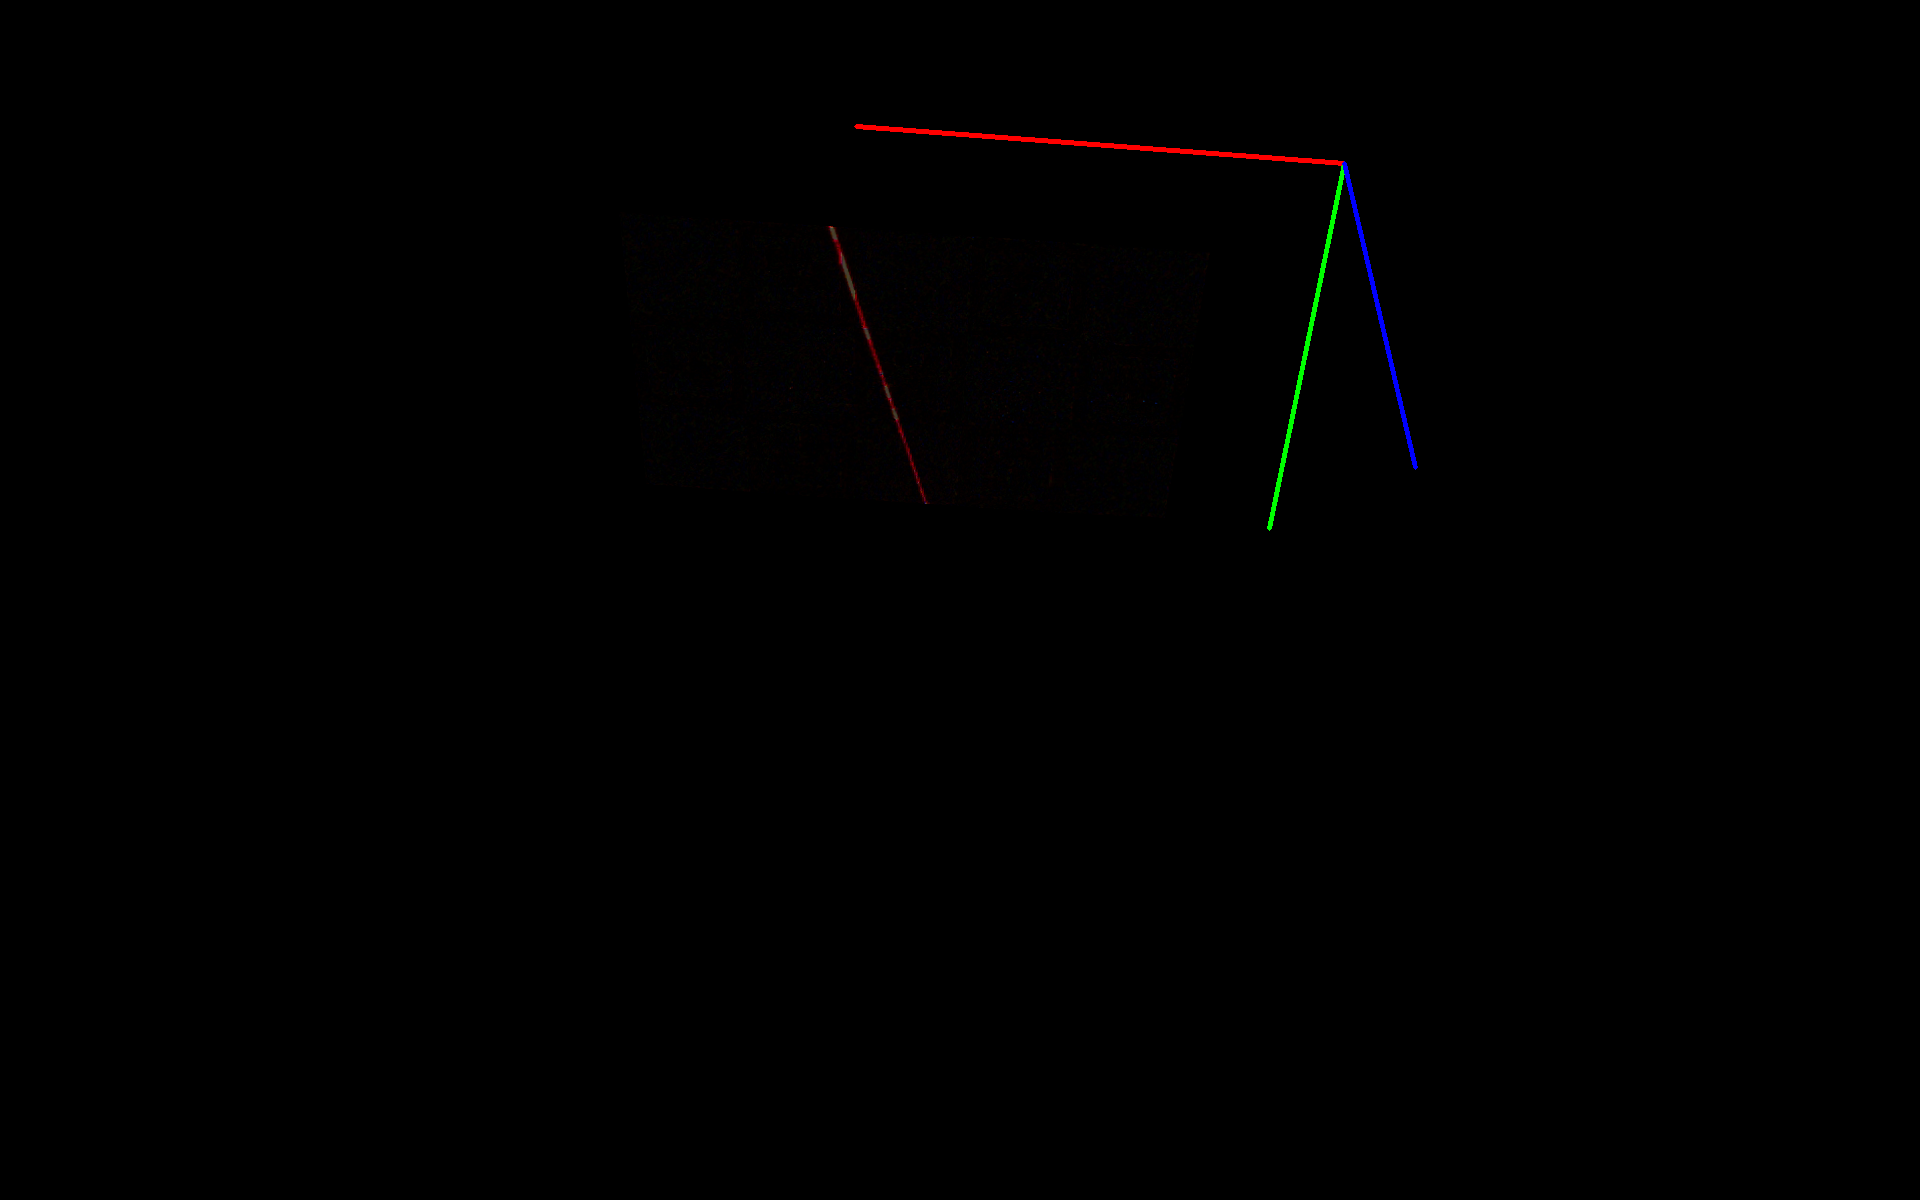
\includegraphics[width=0.49\linewidth]{img/hauptteil/ext-calib/laserline_primary.png}
			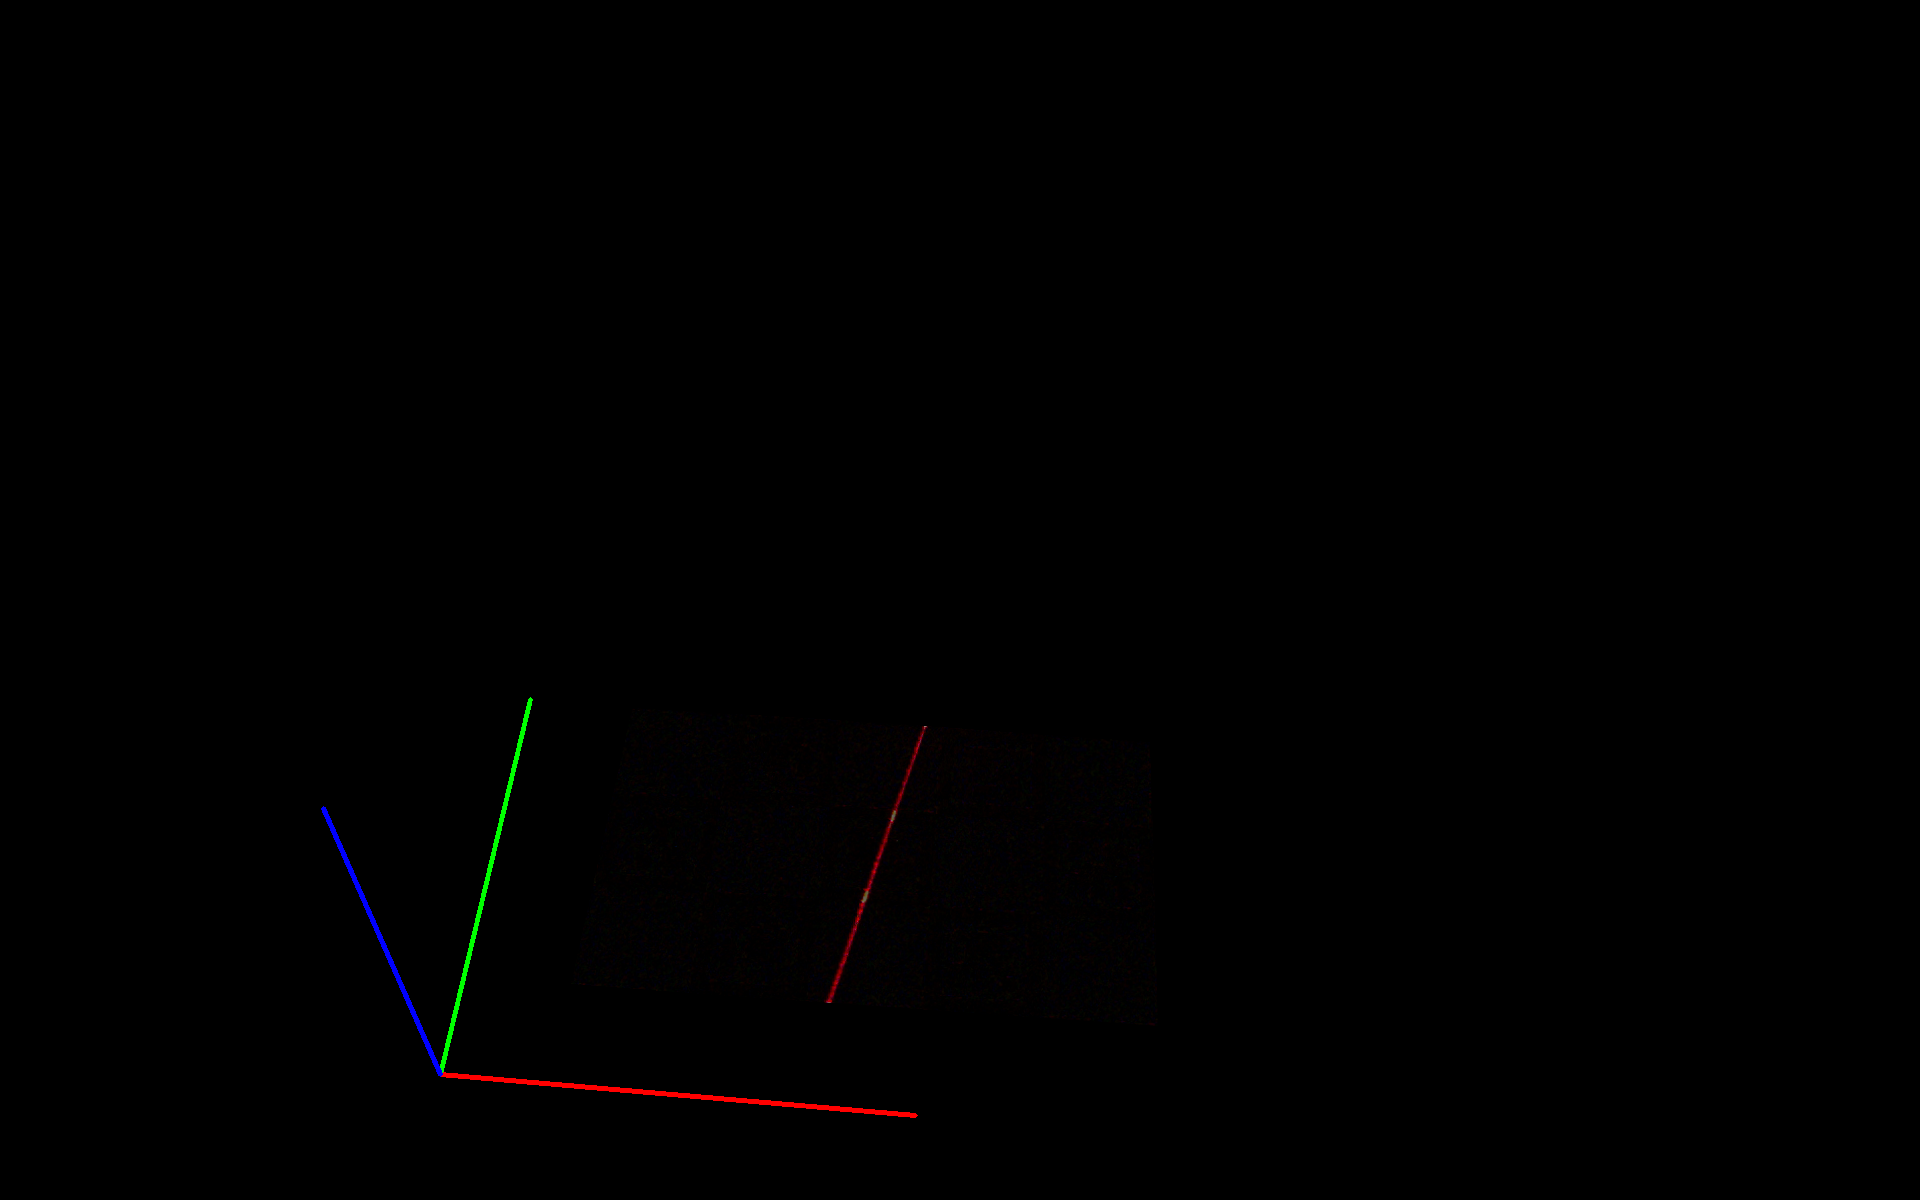
\includegraphics[width=0.49\linewidth]{img/hauptteil/ext-calib/laserline_secondary.png}
			\caption{Herausgearbeitete Laserlinien}
			\label{fig:ext-calib-laserlines}
		\end{figure}
	
		$\underline{Der \; Scale-Factor}$
		
		An diesem Punkt kommt es zum Einsatz der Formel für die 3D-Weltkoordinaten (\ref{eq:basic_trans}). Wie in den Kapitel \ref{chap:transformationen} angemerkt, ist der Scale-Factor noch eine Unbekannte, die gefunden werden muss. Ohne sie wäre die Gleichung noch nicht lösbar. Dieses Problem kann wie folgt umgangen werden. Das Weltkoordinatensystem wird auf das ChArUco-Board gelegt. Die Laserlinie liegt ebenfalls genau auf dem Board. Das bedeutet, dass die Z-Koordinate der Laserlinien-Punkte 0 ist. Zu sehen ist das auch in Abb. \ref{fig:ext-calib-laserlines}. Die Laserlinie liegt in der XY-Ebene. Die Z-Koordinaten der Weltkoordinatenpunkte müssen 0 sein. Mit dem Ausgangspunkt von Gleichung (\ref{eq:pixel_zu_welt}) folgt daraus diese Umstellung:
		
		\begin{equation}
			\begin{aligned}
				p_w &= s \; \vec{a} - \vec{b} \\
				das \; entspricht: \\
				x &= s \; a_x - b_x \\
				y &= s \; a_y - b_y \\
				z &= s \; a_z - b_z \\
				mit \; z &= 0: \\
				0 &= s \; a_z - b_z \\
				s &= \frac{b_z}{a_z}
			\end{aligned}
		\end{equation}
		
		Damit ist die Basistransformationsgleichung lösbar und die 3D-Punkte können errechnet werden. Damit nun eine Ebene in die Punkte gelegt werden kann, müssen alle Punkte in ein einheitliches Koordinatensystem gelegt werden. Durch die bekannten Transformationen ist dies jedoch kein Problem. Zuerst werden mit (\ref{eq:welt_zu_kamera}) und der eigene Rotation und Translation die Weltpunkte der unteren Laserlinie in das Kamerakoordinatensystem transformiert. Danach wird (\ref{eq:kamera_zu_welt}) genutzt, um mit der Rotation und Translation der oberen Laserlinie die Punkte in das obere Koordinatensystem zu bringen. Die folgende Abbildung gilt als Symbolbild.
	
		\begin{figure}[h]
			\centering
			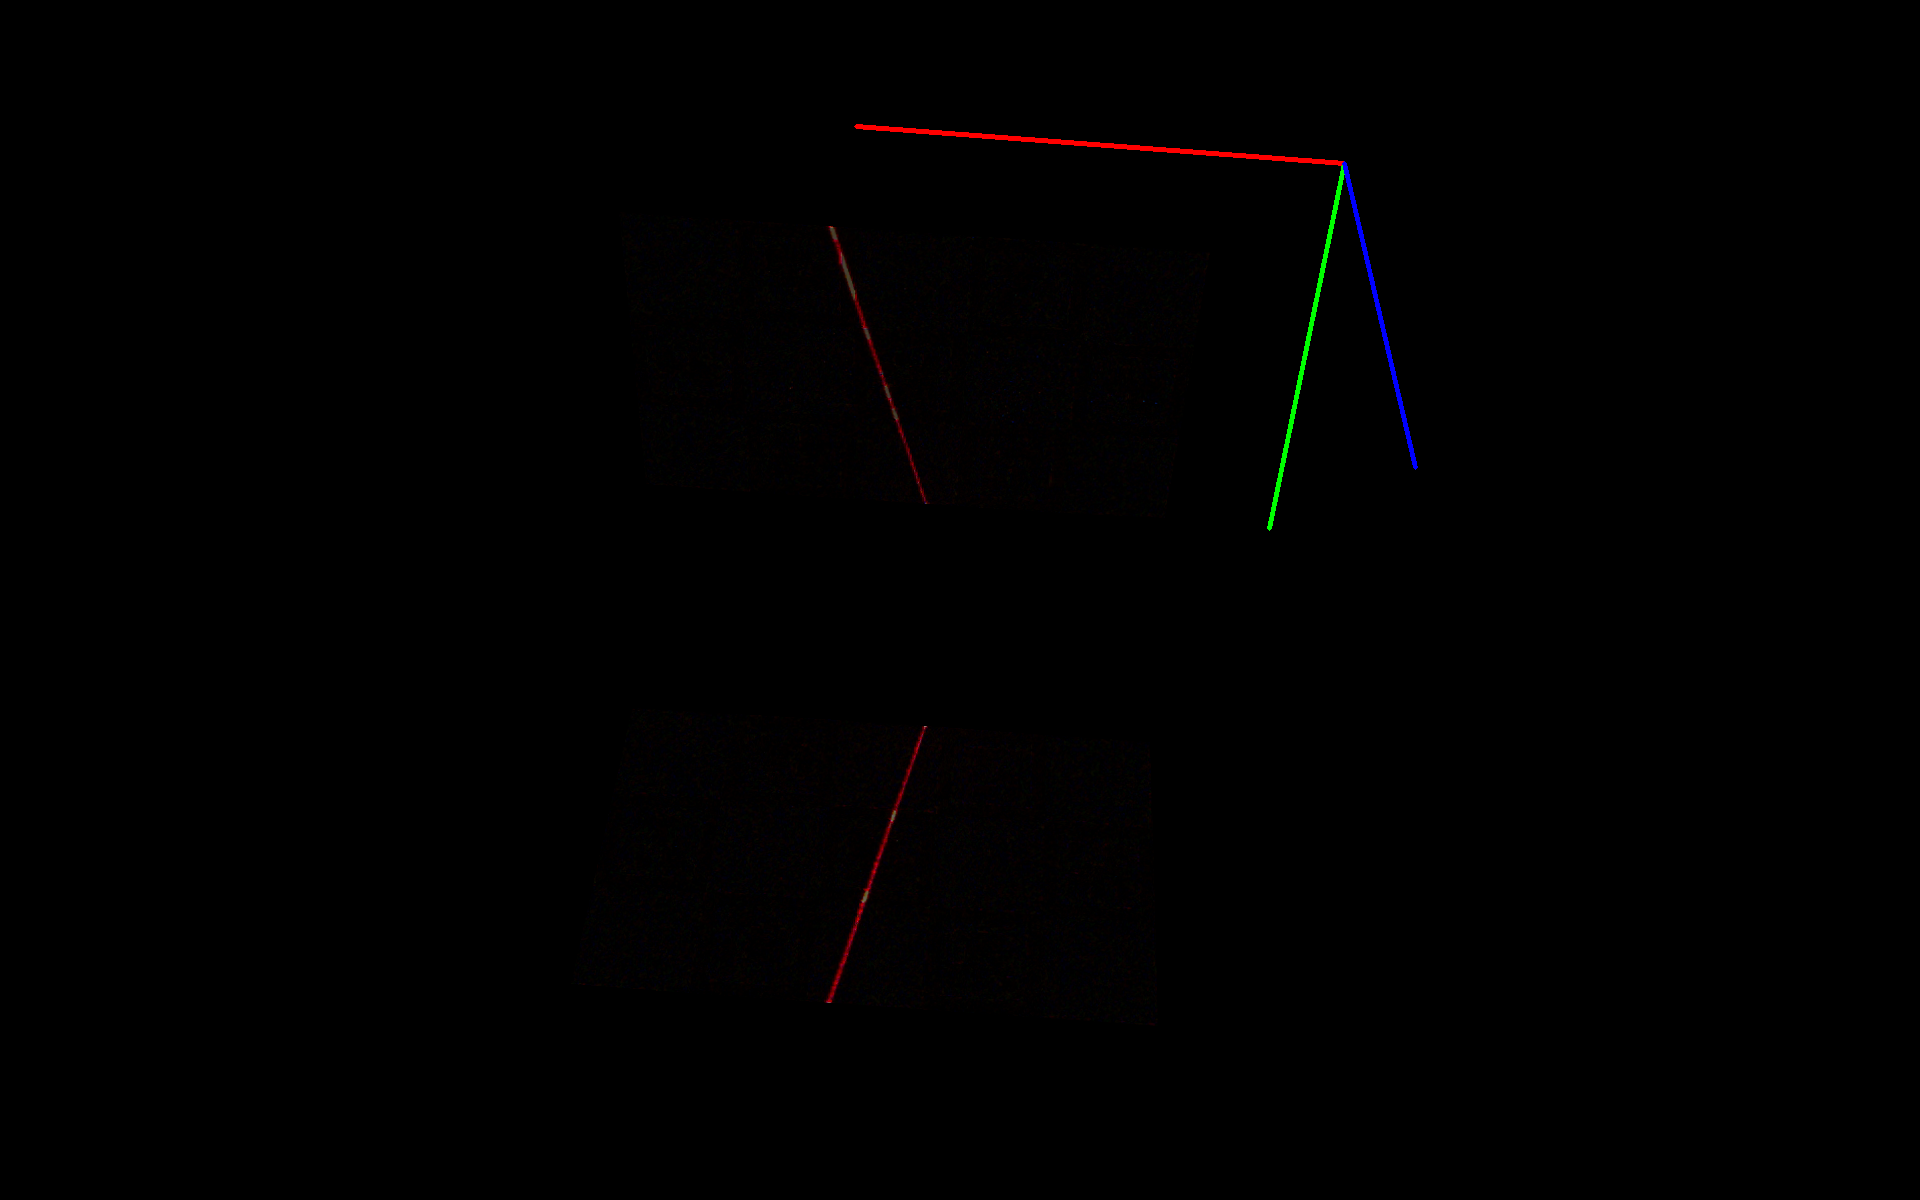
\includegraphics[width=0.85\linewidth]{img/hauptteil/ext-calib/laserline_together.png}
			\caption{Laserlinien in einem Koordinatensystem}
			\label{fig:ext-calib-laserlines-together}
		\end{figure}
	
		$\underline{Das \; Bestimmen \; der \; Ebenengleichung}$
		
		Mit dem letzten Schritt wird die gesuchte Ebenengleichung gefunden. Alle Vorbereitungen sind abgeschlossen. Die richtigen Punkte der zwei nicht parallelen Laserlinien sind in einem einheitlichen Koordinatensystem. Im letzten Schritt muss in diese Punkte eine Ebene gefittet werden. Für einen Ebenen-Fit gibt es diverse Möglichkeiten. Hier wurde sich für die Singular Value Decomposition (SVD) entschieden [svd-t]. Sie ist über die Numpy-Bibliothek in Python implementiert und nutzbar. Wenn man über Numpy den SVD-Algorithmus anwendet, gibt dieser, wie in [svd-t] beschrieben drei Matrizen zurück. Diese heißen U, S und V. Nach [svd-fit] ist die dritte Zeile von U der Normalen-Vektor (\( \vec{n} \)) der passenden Ebene. Ziel ist es eine Ebenengleichung als Koordinatenform zu erhalten. 
		
		\begin{equation}
			\begin{aligned}
				Ax + By +Cz +D &= 0 \\
				\vec{n} &= \begin{pmatrix}
				A \\
				B \\
				C
				\end{pmatrix}
			\end{aligned}
		\end{equation}
		
		Um D zu erhalten kann ein zufälliger Punkt aus den Laserlinien-Punkten ausgewählt werden. Dieser wird dann für x, y und z eingesetzt und D kann errechnet werden. Damit ist das finden der Laser-Ebene abgeschlossen. 
		\label{chap:kalibrierung_extrinsisch}
		
	\subsection{Das Erzeugen einer Punktewolke}
	Mit Beendigung von diesem Schritt ist die komplette Kalibrierung des Lasertriangulationssensors beendet. Bekannt ist nun die Laserebene. Mit Aufnahme der Laserlinie von einer Oberfläche kann nun eine Punktewolke erzeugt werden.
		\subsubsection{Die 3D-Koordinaten}
	Das Erzeugen der Punktewolke fängt ähnlich an, wie die extrinsische Kalibrierung. Die Grundlage sind wieder zwei Bilder. Aus diesen zwei Bildern werden die Laserlinien-Subpixel nach Kapitel \ref{chap:erkennen_der_laserlinie} errechnet. Diese Pixel werden mithilfe der Ebenengleichung in die tatsächlichen 3D-Punkte aus Sicht des Kamerakoordinatensystem umgewandelt. Grundlage sind wieder die Transformationen aus Kapitel \ref{chap:transformationen}. Bei der extrinsischen Kalibrierung konnte der Scale-Faktor (\( s \)) nur mit der Annahme errechnet werden, dass in der X-Y-Ebene mit einer Z-Koordinate gleich 0 liegen. Diese Annahme gilt hier nicht mehr. Sicher ist jedoch jetzt, dass die Punkte in der gefundenen Ebenen-Gleichung liegen. Damit gibt es eine vierte geltende Gleichung und alle Unbekannten können errechnet werden. Die folgende Umstellung erläutert die geltenden Gleichungen. Die Ausgangsbasis ist erneut:
	
	\begin{equation}
		\begin{aligned}
			p_w &= s \; \vec{a} - \vec{b} \\
			das \; entspricht: \\
			x &= s \; a_x - b_x \\
			y &= s \; a_y - b_y \\
			z &= s \; a_z - b_z \\
			f\ddot{u}r \; die \; Ebenengleichung \; gilt: \\
			0 &= Ax + By + Cz + D \\
		\end{aligned}
	\end{equation}
	
	Der ausschlaggebende Wert ist der Scale-Faktor. Dieser kann über ein einsetzten der Koordinaten in die Ebenengleichung bestimmt werden:
	
	\begin{equation}
		\begin{aligned}
			0 &= A(s \; a_x - b_x) + B(s \; a_y - b_y) + C(s \; a_z - b_z) + D \\
			0 &= s \; A \; a_x - A \; b_x + s \; B \; a_y - B \; b_y + s \; C \; a_z - C \; b_z + D \\
			0 &= s \; A \; a_x + s \; B \; a_y + s \; C \; a_z - A \; b_x - B \; b_y - C \; b_z + D \\
			0 &= s(A \; a_x + B \; a_y + C \; a_z) - (A \; b_x + B \; b_y + C \; b_z) + D \\
			\vec{n} &= \begin{pmatrix}
			A \\
			B \\
			C
			\end{pmatrix} \\
			0 &= s(\vec{n} \cdot \vec{a}) - (\vec{n} \cdot \vec{b}) + D \\
			s &= \frac{\vec{n} \cdot \vec{b} - D}{\vec{n} \cdot \vec{a}}
		\end{aligned}
	\end{equation}
	
	Der Scale-Faktor ist damit bekannt und die Koordinaten x, y und z können bestimmt werden. Wichtig hierbei ist, dass die Ebenengleichung in einem Weltkoordinatensystem liegt. Dementsprechend müssen die errechneten 3D-Punkte mit der bekannten Transformation (\ref{eq:welt_zu_kamera}) von dem Weltkoordinatensystem zum Kamerakoordinatensystem transformiert werden.
	
	\subsubsection{Das Finden der Farbinformationen}
	
	Zusätzlich gefordert zu den reinen 3D-Informationen waren auch Farbinformationen. Diese können ebenfalls über das grundlegende Bild-Paar gefunden werden. Das Bild, welches ohne das Einschalten des Lasers aufgenommen wird, beinhaltet die gesuchten Farbinformationen. Gesucht wird nur nach der Farbe an der richtigen Stelle. Die Pixel-Werte der Laserlinie sind bekannt. In dem Ursprungsbild muss an genau der Stelle, an der sich ein Laserpixel befindet die Farbe ausgelesen werden und für den jeweiligen Punkt abgespeichert werden. Problem hierbei ist, dass die Laserpixel Subpixel sind und sich demnach zwischen zwei Pixeln befinden. Für die endgültige Farbe werden dann die zwei umrandenden Pixel gewichtet zusammengerechnet.
	\begin{figure}
		\centering
		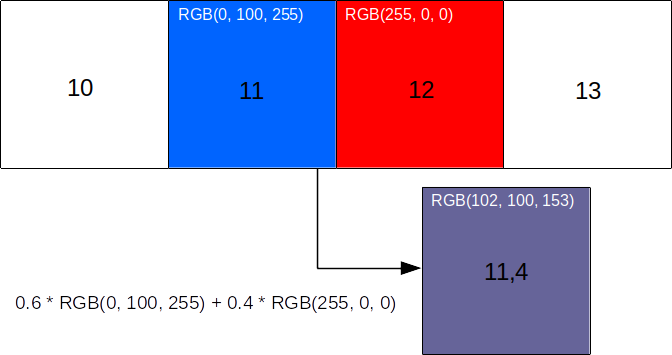
\includegraphics[width=0.85\linewidth]{img/hauptteil/bildverarbeitung/weighted_pixel.png}
		\caption{Gewichtete Pixel für den x-Wert 11,4}
		\label{fig:weighted_pixel}
	\end{figure}
	Die Abbildung \ref{fig:weighted_pixel} zeigt den Vorgang an einem simplen Beispiel für ein Subpixel in einer beliebigen Reihe (y-Wert) mit einem beispielhaften x-Wert von 11,4. Der nähere Pixel (11) fließt mit höheren Gewicht in die resultierende Farbe ein, als der Pixel weiter weg (12). Die y-Werte der Pixel können keinen ungeraden Wert beinhalten, da der Algorithmus zum Finden der Laser-Pixel (Kapitel \ref{chap:erkennen_der_laserlinie}) jede Pixel-Zeile im Bild durchläuft und dort einen neuen x-Wert errechnet.
	
	Dieser komplette Vorgang transformiert genau eine aufgenommene Laserlinie in eine Punktewolke. Um eine ganze Oberfläche zu rekonstruieren muss sich die Position der des Sensors um eine bekannte Länge und Richtung verschieben. Die neu Punktewolke, die aus der neu aufgenommenen Laserlinie resultiert, muss dann entsprechend zu einer Gesamt-Punktewolke ergänzt werden. Um die neuen Punkte korrekt einzufügen , ist es zwingend erforderlich, dass die Bewegung genau bekannt ist. 
	
	\newpage
	
	\subsection{Aufbau / Hardware}
	Damit das Scannen einer kompletten Oberfläche getestet werden kann, wurde ein Versuchsaufbau angefertigt.
	
	\label{chap:aufbau_hardware}
	
	\newpage
	
	\subsection{Aufbau / Software}
	Die Software des Lasertriangulationssensor gliedert sich in zwei Bereiche. Zum einen wurde eine Python-Bibliothek entwickelt. Diese wurde Objektorientiert mit diversen Klassen, die den Lasertriangulationssensor repräsentieren entwickelt. Grundlegende Aufgabe der Python-Bibliothek sind die elementaren Berechnungen, um eine Punktewolke aus einem Bild-Paar zu erhalten. Das bedeutet, dass ein Konstrukt erstellt werden kann, welches Kalibriert werden kann und darauf folgend Punktewolken liefert. \newline
	Der andere große Bereich ist die Umsetzung in ROS2. ROS2 liefert das Betriebssystem des Scanners. Alle verschiedenen Elemente sollen zu einem Gesamtprodukt zusammengefügt werden. Dazu gehört die Ansteuerung der Kamera und des Lasers. Schwerpunkt ist auch die Kommunikation zwischen einzelnen Elementen. Beispiele sind dabei das Aufnehmen der Bilder für die Kalibrierung oder das Erstellen der Punktewolke und die Weiterleitung an die entsprechenden Methoden aus den Klassen der Python-Bibliothek.
		\subsubsection{Python (Bibliothek)}
		Die Python-Bibliothek besteht grundlegend aus vier Klassen. Die Scanner-, Kamera-, Laser-, und LaserLine-Klasse. Dabei ist die Scanner-Klasse die volle Representation des Lasertriangulationssensors, die in ROS2 eingebunden wird.
		
		\begin{figure}[h]
			\centering
			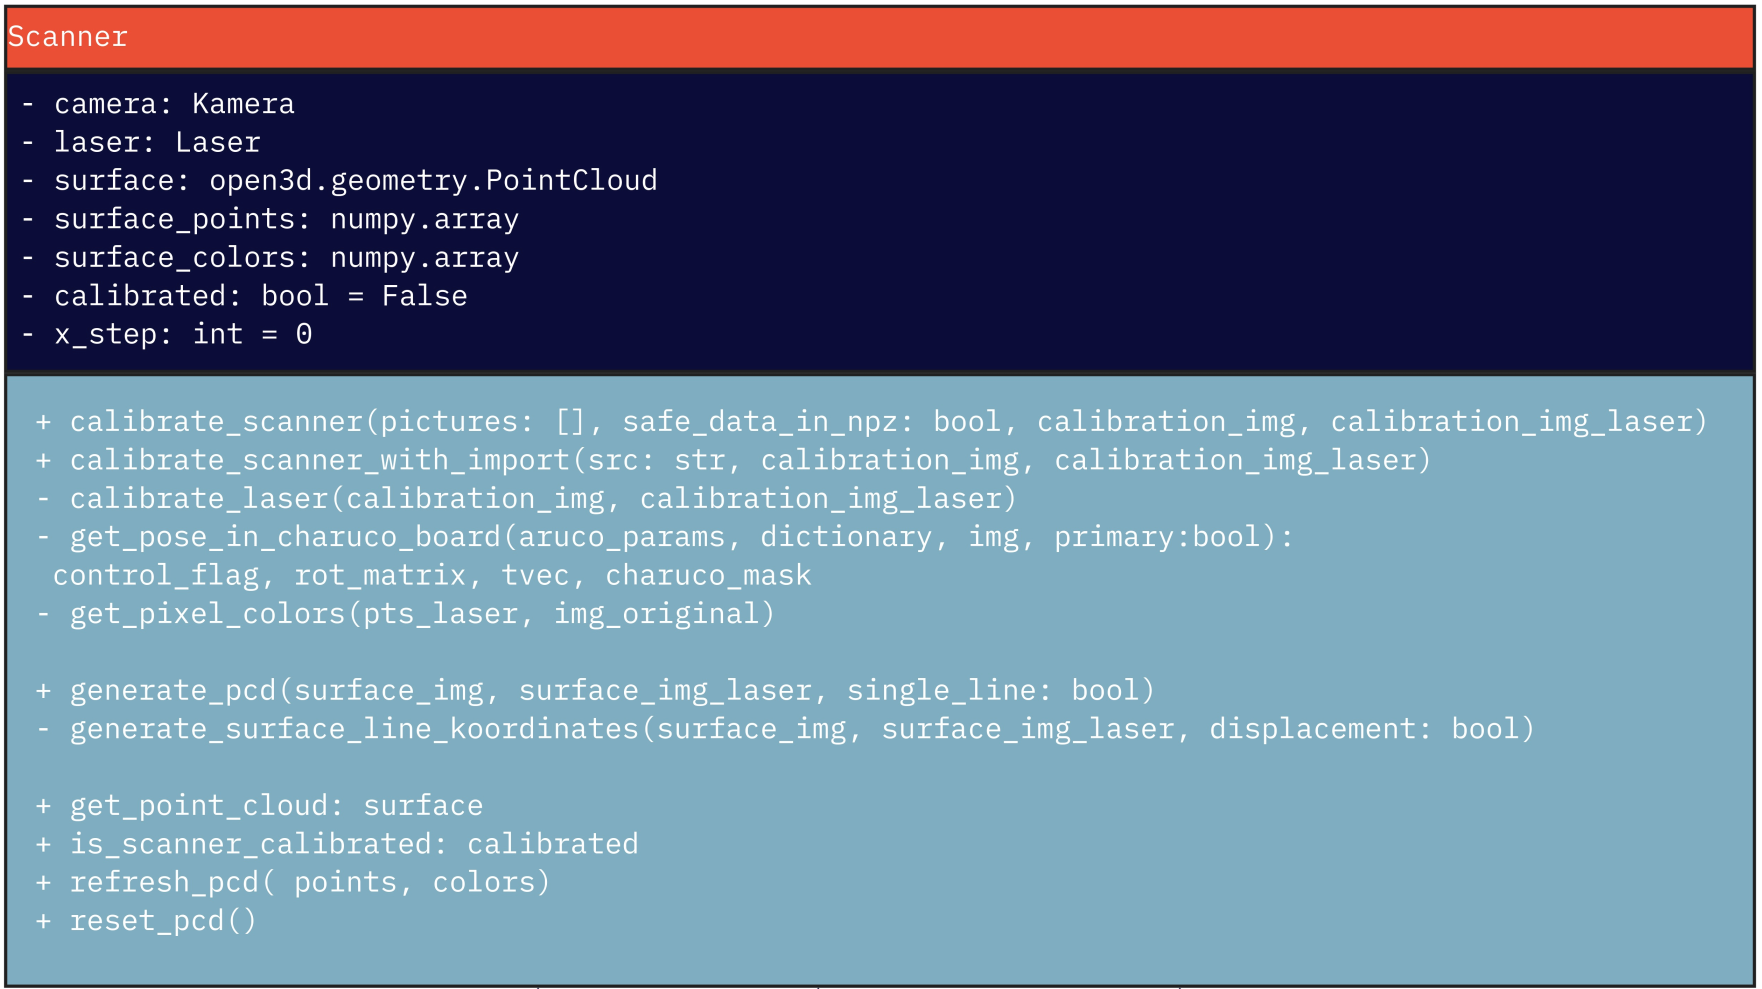
\includegraphics[width=0.85\linewidth]{img/hauptteil/software/Scanner_UML.png}
			\caption{Die Scanner-Klasse als UML-Diagramm}
			\label{fig:scanner_uml}
		\end{figure}
		Der Scanner beschreibt den Lasertriangulationssensor. Er besitzt eine Kamera und einen Laser. Zusätzlich wird als Variable die Punktewolke der Oberfläche und auch direkt deren Punkte und Farben abgespeichert. Hinzu kommt ein Boolean-Flag um zu kennzeichnen, ob der Scanner kalibriert ist. Der xStep ist für den Versuchsaufbau wichtig. Über die Liniarführung wird das Objekt in x-Richung unter dem Sensor durch bewegt. Die jeweiligen Millimeter-Schritte müssen entsprechend einbezogen werden. Dazu wird diese Variable genutzt. \newline
		Zusätzlich stellt die Scanner-Klasse die grundlegenden Methoden, die die Funktionalität des Triangulationssensors wieder spiegel, zur Verfügung. Diese umfassen zum einen das komplette kalibrieren des Scanners. Dazu wird eine Liste von Bildern für die intrinsische Kalibrierung und ein Bildpaar des ChArUco-Boards für die extrinsische Kalibrierung benötigt. Hinzu kommt eine abgewandelte Version der Kalibrier-Methode, in der die intrinsische Kalibrierung durch das Importieren der Kameradaten ersetzt wird. Hinzu kommt die Methode zum Erstellen einer Punktewolke. Sie bekommt ein entsprechendes Bildpaar von der Oberfläche übergeben und errechnet die Punktewolke. Wenn der Scanner sich gerade in einem Scanvorgang befindet wird die neue Punktewolke entsprechend an die gesamte Punktewolke angehängt. Die Scanner-Klasse besitzt zusätzlich noch Hilfsmethoden die Zugriff von außen auf den Scanner Status und die Punktewolke geben oder die Punktewolke selbst erneuern oder aktualisieren.
		
		\begin{figure}[h]
			\centering
			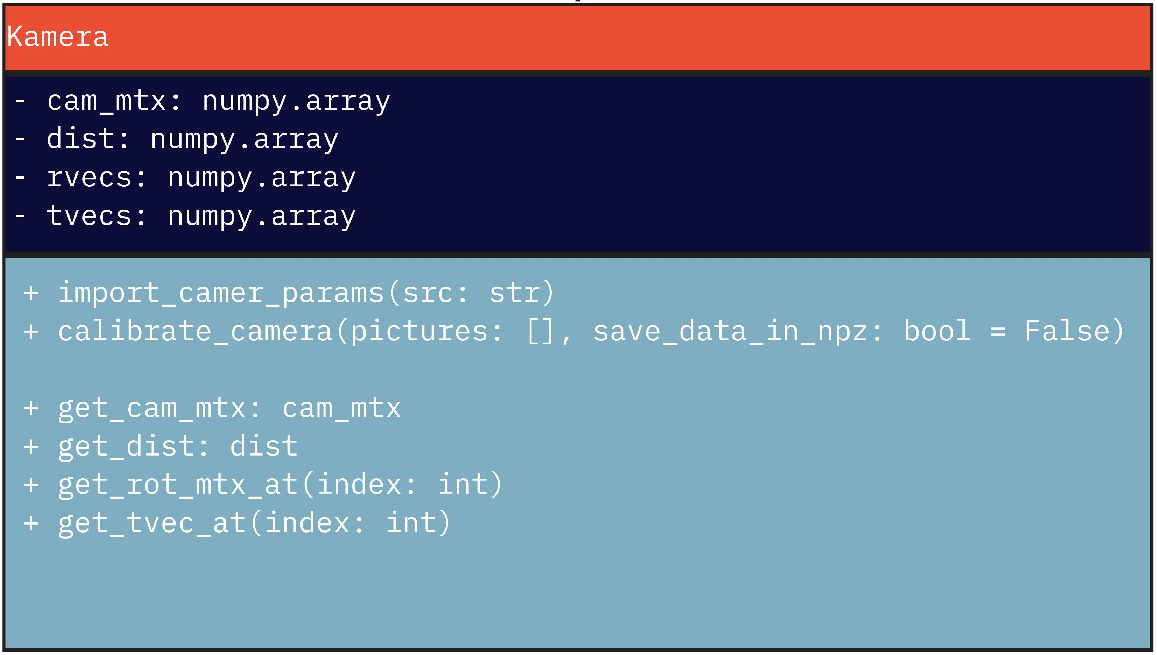
\includegraphics[width=0.7\linewidth]{img/hauptteil/software/Kamera_UML.png}
			\caption{Die Kamera-Klasse als UML-Diagramm}
			\label{fig:kamera_uml}
		\end{figure}
		Die Kamera selbst besitzt auch eine Repräsentation in Form einer Klasse. Diese Klasse fungiert als Speicher für die Kameradaten. Gespeichert werden die Kamera-Matrix die Distortion-Koeffizienten und die Rotationsmatrizen sowie die Translationsvektoren der Bilder von der intrinsischen Kalibrierung. Also alle Daten, die aus der intrinsische Kalibrierung hervorgehen. Hierbei ist wichtig hervorzuheben, dass die Klasse keine Bilder aufnehmen kann bzw kein Zugriff auf die tatsächliche Kamera im Triangulationssensor hat. Sie is lediglich für das Ablegen der Daten und die intrinsische Kalibrierung zuständig.
		\newpage
		\begin{figure}[h]
			\centering
			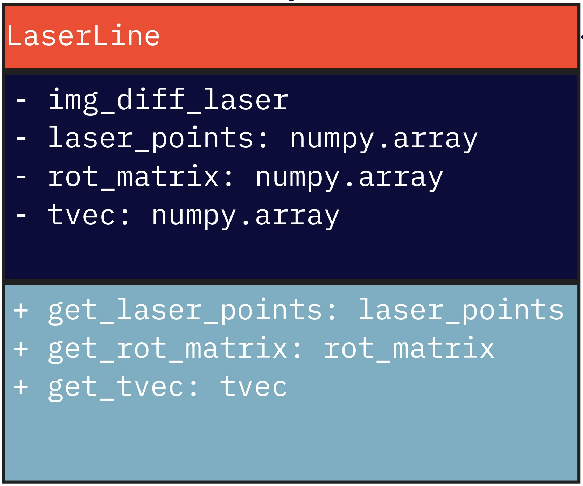
\includegraphics[width=0.35\linewidth]{img/hauptteil/software/LaserLine_UML.png}
			\caption{Die LaserLine-Klasse als UML-Diagramm}
			\label{fig:laser_line_uml}
		\end{figure}
		Die Klasse LaserLine beschreibt eine aufgenommene Laserlinie. Information die dafür als Variablen gespeichert werden sind das Differenz-Bild, die errechneten 3D-Punkte der Linie und die entsprechende Rotation und Translation zu dem Weltkoordinatensystem, in dem sich die Laserlinie befindet. Zum initialisieren der LaserLine-Klasse wird das aufgenommene Bildpaar und die Rotation und Translation zu dem jeweiligen Weltkoordinatensystem benötigt. Die Klasse errechnet dann noch im Konstruktor die Bild-Differenz und die Laserlinienpunkte.
		
		\begin{figure}[h]
			\centering
			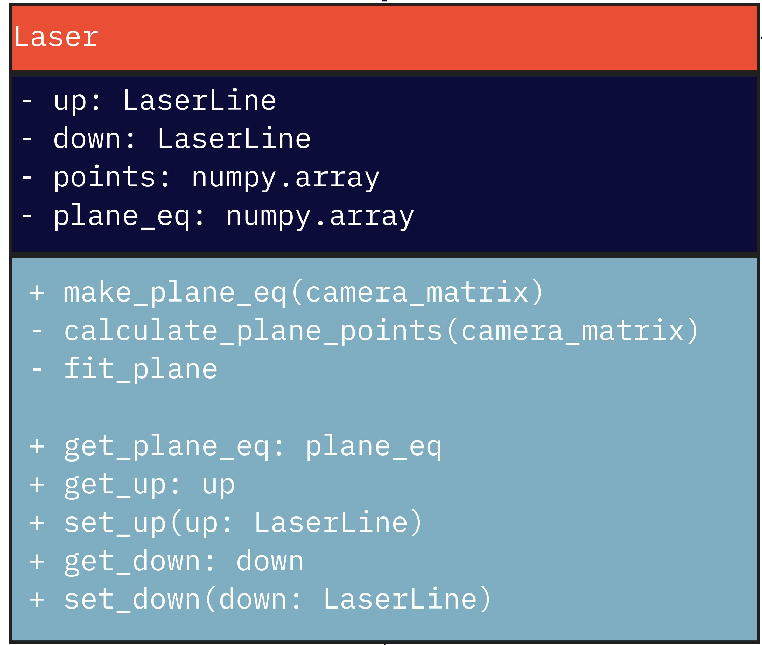
\includegraphics[width=0.35\linewidth]{img/hauptteil/software/Laser_UML.png}
			\caption{Die Laser-Klasse als UML-Diagramm}
			\label{fig:laser_uml}
		\end{figure}
		So wie die Kamera-Klasse die Daten der intrinsischen Kalibrierung beinhaltet, beinhaltet die Laser-Klasse die Daten der extrinsischen Kalibrierung. Dazu benötigt sie zwei Laserlinien der Klasse LaserLine, die zur Unterscheidung als \glqq oben\grqq{} und \glqq unten\grqq{} definiert sind. Aus diesen kann die Ebenengleichung bestimmt werden. Dazu wird eine eigene Methode bereitgestellt in der erst die Punkte in ein einheitliches Koordinatensystem zusammengefasst und dann eine Ebene an die Punkte gefittet wird. Die vereinheitlichten Punkte und die Ebenengleichung werden von der Klasse gespeichert.
		\newpage
		\begin{figure}[h]
			\centering
			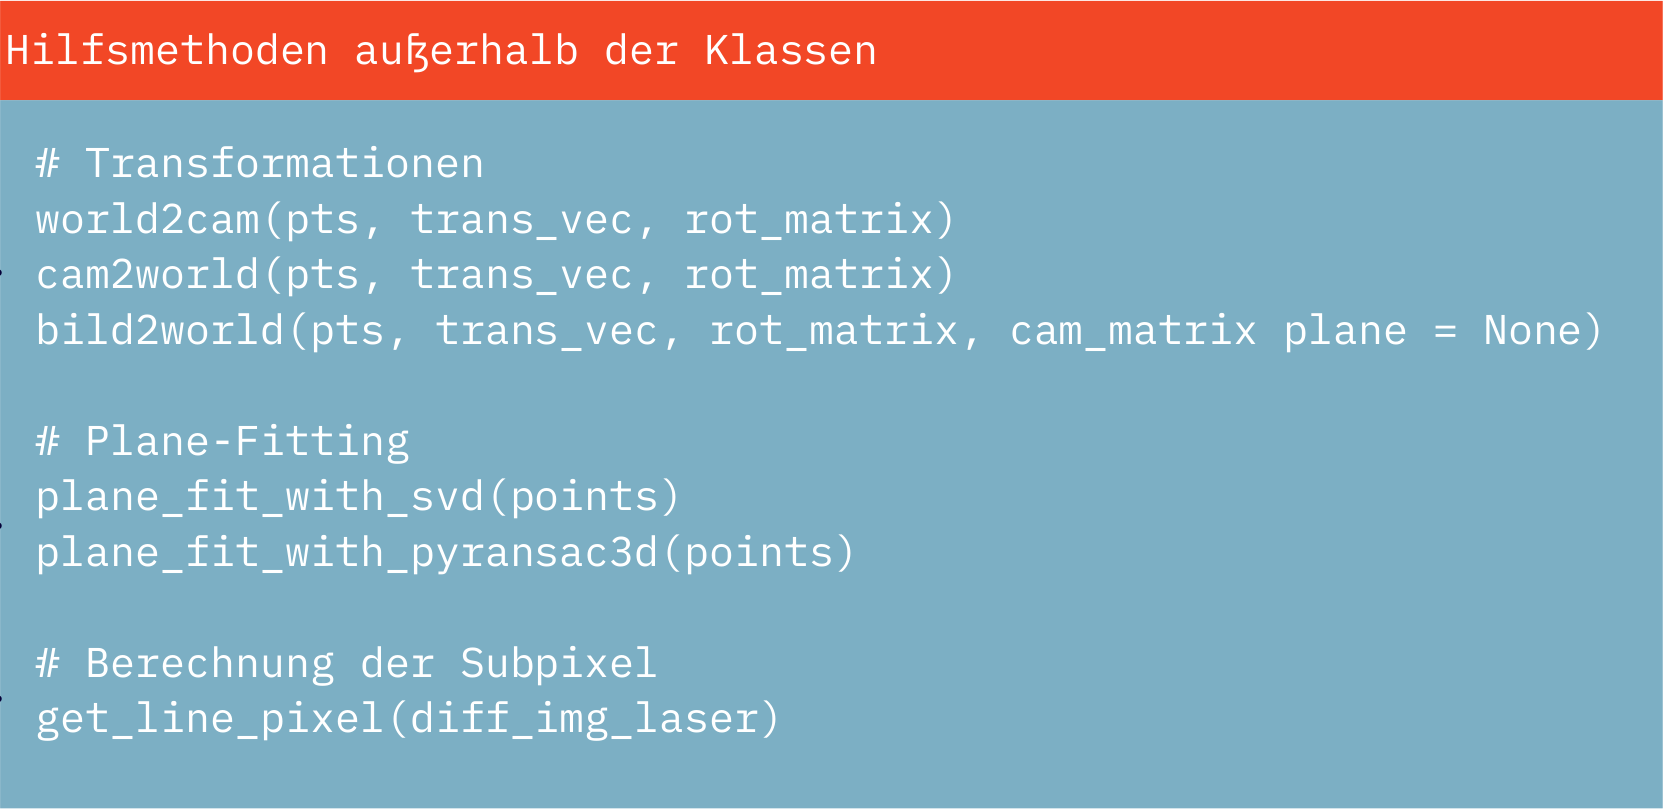
\includegraphics[width=0.7\linewidth]{img/hauptteil/software/Hilfsmethoden_UML.png}
			\caption{Die Hilfsmethoden ohne Zugehörigkeit zu einer Klasse}
			\label{fig:hilfsmethoden_uml}
		\end{figure}
		Zusätzlich zu den vier beschriebenen Klassen gibt es Hilfsmethoden, die nicht konkret zu einer Klasse gehören. Das bedeutet, dass sie nicht nur von einer Klasse benutzt werden, sondern von verschiedenen Klassen an verschiedenen Stellen aufgerufen werden. Diese Methoden umfassen die Transformationen zwischen den Koordinatensystemen, die Methoden für das Plane-Fitting und die Berechnung der Subpixel aus einem Differenz-Bild.
		
		Die gesamte Darstellung des UML-Diagramm befindet sich im Anhang unter Abbildung \ref{fig:uml_all}.
		
		\subsubsection{ROS2}
		
		Übergeordnet über der Python-Bibliothek befindet sich die ROS2-Implementierung, mit der letztendlich der Triangulationssensor bedient wird. Mit ROS2 erstellt man sogenannte \textbf{Nodes}, die über verschiedene Möglichkeiten miteinander Kommunizieren können. Dazu gehören zum einen \textbf{Services}. Services sind am ehesten mit Methoden einer Klasse zu vergleichen. Eine Node stellt ein Service bereit. Dieser kann aufgerufen werden und man erhält eine Response zurück. Der Triangulationssensor selbst ist auch über Nodes umgesetzt. Dabei sind die beiden ausschlaggebenden Nodes sind die Scanner-Node und die Kamera-Node. Die Scanner-Node enthält die vorgestellte Python-Bibliothek und damit eine Instanz von der Scanner-Klasse. Die Instanzen von der Scanner-Klasse selbst, also der Laser und die Kamera sind nach Initialisierung noch nicht mit Daten gefüllt. Das liegt daran, dass die Kalibrierung noch nicht stattgefunden hat. Dazu gibt es die Kamera-Node, die nun konkrete Bilder liefern kann. Die Kamera-Node hat Zugriff auf die Pypylon-Bibliothek [pypylon] und damit auf die Repräsentation der Basler-Kamera. Die Node beinhaltet eine Funktion, die das gewünschte Bildpaar liefern kann. Da der Linienlaser selbst über den Output der Kamera gesteuert wird, kann dieser auch direkt in der Kamera-Node angesprochen werden. So stellt die Kamera ein Service bereit, der ein Bildpaar aufnimmt und dieses an den Scanner weiterleiten kann. Diese Kommunikation funktioniert in ROS2 über \textbf{Topics}. Topics beschreiben eine Nachricht. Eine Node hat die Möglichkeit eine Nachricht über ein gewähltes Topic zu veröffentlichen (publish). Ebenfalls gibt es die Möglichkeit , dass eine Node Nachrichten über einem gewählten Topic empfängt (subscribe). Nachdem die geforderten Bilder von der Kamera veröffentlicht wurden, ist der Service damit fertig. Ein Service kann bei ROS2 ein Feedback zurück geben. Diese Möglichkeit wird hier genutzt, damit die Kamera zeigen kann, dass die Bilder erfolgreich aufgenommen und veröffentlicht wurden. In der Kommunikation muss zusätzlich festgehalten werden, welcher Typ an Nachricht benutzt werden soll. In ROS2 wird das über einen \textbf{Message}-Type realisiert. Hierbei kann man selbst eine Message erstellen oder man benutzt vorgefertigte, die von ROS2 bereitgestellt werden. Für ein Bild gibt es einen vorgefertigten Message-Type. Da jedoch zwei Bilder auf einmal geschickt werden sollen, wurde hier ein eigener Typ (img\_pair.msg) erstellt. Ähnlich verhält es sich bei dem Schicken der Kalibrierungsbilder für die intrinsische Kalibrierung. Hier wird ein Message-Type erstellt, der eine Liste an Bildern beinhaltet (cam\_calib\_imgs.msg). Die Kamera nimmt demnach bei einem Aufruf des Services die Bilder auf und veröffentlicht sie über das jeweilige Topic. Der Scanner ist ein Subscriber zu diesem Topic und empfängt sie. Dabei wird in der Node eine Callback-Function aufgerufen, die auf dieses Empfangen reagiert. Der Scanner selbst speichert die für die Kalibrierung gesendeten Bild erst einmal nur ab. Die Node bietet eine eigenen Service bereit, der den Scanner Kalibriert. Dazu werden die Methoden, die die Scanner-Klasse bereitstellt genutzt. Überprüft wird hierbei
		
	\subsection{Qualitative Ergebnisse}
	
	\subsection{Evaluation}
		\subsubsection{Testen von Genauigkeit}
		\subsubsection{Fehler}
		\subsubsection{Probleme und Schwierigkeiten}
			\label{chap:probleme_schwierigkeiten}